% !TeX root = RJwrapper1.tex
\title{mtarm: Bayesian Analysis of Multivariate Threshold Autoregressive Models in R}
\author{by L.H. Vanegas, S.A. Calderón V. and L.M. Rond\'on}

\maketitle

\abstract{
This paper introduces mtarm, an R package for Bayesian estimation, inference, and forecasting in multivariate Threshold Autoregressive (TAR) models. The package supports both standard m-step-ahead forecasting from a single model fit and rolling-origin forecast evaluation without repeated model re-estimation. These models provide a flexible framework for analyzing nonlinear multivariate time series and encompass important special cases such as multivariate Self-Exciting Threshold Autoregressive (SETAR) models and Vector Autoregressive (VAR) models. The package supports a broad class of innovation distributions beyond the Gaussian assumption, including the Student-t, slash, symmetric hyperbolic, Laplace, contaminated normal, skew-normal, and skew-t distributions, thereby accommodating heavy tails, skewness, and other forms of non-normality frequently observed in practice. Inference is performed within a Bayesian framework using a Markov chain Monte Carlo (MCMC) algorithm that jointly estimates all model parameters, except for the number of regimes. The resulting posterior samples can be readily summarized, visualized, and diagnosed through integration with the coda package. For model assessment and selection, mtarm implements several predictive and information-based criteria, including the Deviance Information Criterion (DIC), the Watanabe--Akaike Information Criterion (WAIC), the log-score, the Continuous Ranked Probability Score (CRPS), the Energy Score (ES), and a variety of forecast accuracy measures. Additional functionality includes graphical goodness-of-fit diagnostics and simulation of multivariate TAR processes. The capabilities of mtarm are illustrated through the analysis and forecasting of two real multivariate time series.
}

\section{Introduction}
Threshold Autoregressive (TAR) models were originally introduced by \cite{tong1978threshold,tong1983threshold} and have become one of the most widely used frameworks for modeling nonlinear dynamics in time series. By allowing the autoregressive structure to vary across regimes defined by threshold variables, TAR models can effectively capture structural changes, asymmetric adjustments, and regime-switching behavior. In contrast, linear autoregressive (AR) models—obtained as a special case of a TAR model with a single regime—are generally unable to adequately represent such features. Owing to their flexibility, TAR models have been successfully applied in a wide range of fields. In economics, they have been used to model gross national product (GNP) growth, unemployment, and inflation rates; in finance, to analyze stock returns and insurance pricing; in hydrology, to describe river flow dynamics; and in ecology, to study annual records of lynx trapping, among many other applications (see \cite{T90,hansen2011threshold,Chen2011,TONG2011,TONG2015}).

Within the TAR family, several important extensions have been developed. In the univariate setting, these include the incorporation of moving average components through Threshold Autoregressive Moving Average (TARMA) models \citep{T90}, the introduction of conditional heteroscedasticity via Threshold Autoregressive Conditional Heteroscedastic (TAR-ARCH) models \citep{LIU1997279}, and recent advances in testing for threshold effects based on supremum Lagrange multiplier procedures \citep{Goracci2023,GIANNERINI2024105379}. In the multivariate context, \cite{T98} introduced the Multivariate Threshold Autoregressive (MTAR) model, which was subsequently extended to the Threshold Vector Autoregressive Moving Average (TVARMA) framework by \cite{Niglio2015}. More recently, \cite{VANEGAS2025} further generalized the TAR models by allowing for non-Gaussian error distributions.

Despite the theoretical importance and wide applicability of TAR-type models, their statistical implementation in {\tt R} remains relatively limited. For example, the package \CRANpkg{tsDyn} \citep{stigler2018tsdyn} provides a well-established framework for nonlinear time series analysis, including Self-Exciting Threshold Autoregressive (SETAR) models. Estimation is based on conditional least squares, a frequentist approach that typically assumes Gaussian innovations and determines threshold values through grid-search optimization, which can become computationally demanding in the presence of multiple thresholds or high-dimensional settings. Likewise, the package \CRANpkg{NTS} \citep{liu2020nts} supports the estimation of multivariate TAR models and includes tools for simulation, prediction, and model identification. However, its methodology is also rooted in a frequentist framework, relies on Gaussian innovation assumptions, and offers limited flexibility for accommodating alternative error distributions. More recently, the package \CRANpkg{tseriesTARMA} \citep{tseriesTARMA} expanded the range of available nonlinear time series tools by implementing threshold ARMA models under a frequentist paradigm. In contrast, the package \CRANpkg{BAYSTAR} \citep{BAYSTAR} adopts a Bayesian perspective, providing inference for univariate TAR models with flexible prior specifications. Nevertheless, its scope is restricted to the univariate case.

However, existing software solutions remain fragmented, typically focusing exclusively on either univariate or multivariate time series. Moreover, most available implementations are restricted to two-regime models and do not naturally accommodate more complex multi-regime structures. To the best of our knowledge, the \CRANpkg{NTS} package currently provides the most comprehensive framework for handling both univariate and multivariate TAR models with multiple regimes. However, its inferential procedures are limited by Gaussian innovation assumptions and do not support the broad class of non-Gaussian error distributions frequently encountered in practice. Such distributions arise naturally in applications involving financial returns, river flows, unemployment rates, and many other phenomena characterized by nonlinear and regime-dependent dynamics. As a result, there is a growing demand for a unified statistical framework that can simultaneously accommodate univariate and multivariate TAR models, allow for multiple regimes, and provide the flexibility to model non-Gaussian innovations. Such a framework would be particularly valuable in fields such as finance, economics, hydrology, and other disciplines where departures from normality and regime-switching behavior are common.

To address these limitations, we introduce \CRANpkg{mtarm}, a new {\tt R} package for the Bayesian analysis of multivariate TAR-type models. The package is built upon the methodology developed by \cite{VANEGAS2025} and extends the current {\tt R} ecosystem by providing a flexible and unified framework for Bayesian inference in TAR models. Specifically, \CRANpkg{mtarm} contributes in the following ways:
\begin{itemize}
\item {\bf Unified modeling framework.} The package supports the estimation of multivariate TAR models and several important special cases, including Self-Exciting Threshold Autoregressive (SETAR) models and Vector Autoregressive (VAR) models, together with their univariate counterparts. This unified framework facilitates model comparison and allows users to seamlessly transition between linear and nonlinear specifications.

\item {\bf Flexible innovation distributions.} In contrast to most existing implementations, which are restricted to Gaussian innovations, \CRANpkg{mtarm} accommodates a broad class of multivariate distributions, including the Student-$t$, slash, symmetric hyperbolic, Laplace, contaminated normal, skew-normal, and skew-$t$ distributions. These distributions provide increased robustness to heavy tails, skewness, and other forms of non-normality commonly observed in real-world applications.

\item {\bf Bayesian inference and forecasting.} All aspects of estimation, inference, and prediction are carried out within a Bayesian framework. Model parameters are estimated jointly through a Markov chain Monte Carlo (MCMC) algorithm, eliminating the need for the sequential grid-search procedures commonly employed in frequentist approaches. This strategy yields a coherent quantification of uncertainty through posterior distributions and naturally supports probabilistic forecasting. The package supports both standard $m$-step-ahead forecasting from a single model fit and rolling-origin forecast evaluation without repeated model re-estimation.
\end{itemize}

The remainder of the paper is organized as follows. Section 2 presents the statistical framework for multivariate TAR models and summarizes the Bayesian methodology implemented in \CRANpkg{mtarm}. Section 3 describes the package architecture and its main functionalities through an empirical application involving rainfall and the flows of two rivers in Colombia. Section 4 further illustrates the use of the package through a second empirical application involving precipitation, temperature, and the flows of two rivers in Iceland.

\section{Theoretical framework}
\subsection{Model formulation}\label{mf}

Let $\{\bm{Y}_t\}_{t\geq 1}$ be the $k$-dimensional time series of interest (output),
$\{\bm{X}_t\}_{t\geq 1}$ the $r$-dimensional time series of exogenous covariates, and
$\{Z_t\}_{t\geq 1}$ the one-dimensional threshold time series.
We say that $\{\bm{Y}_t\}_{t\geq 1}$ follows a multivariate Threshold Autoregressive (TAR)
model with $l$ regimes, denoted ${\rm TAR}(l;\bm{p},\bm{q},\bm{d})$, if
\begin{equation}\label{mtar}
\bm{Y}_t=\sum_{j=1}^l I(Z_{t-h}\in(c_{j-1},c_j])\Big(\!\bm{\phi}_0^{^{(j)}}\!\bm{D}_t
+\sum_{i=1}^{p_j}\bm{\phi}_i^{^{(j)}}\bm{Y}_{t-i}
+\sum_{i=1}^{q_j}\bm{\beta}_i^{^{(j)}}\bm{X}_{t-i}
+\sum_{i=1}^{d_j}\bm{\delta}_i^{^{(j)}}Z_{t-i}
+\bm{\epsilon}_{t_j}\!\Big),
\end{equation}
where $\bm{p}=(p_1,\ldots,p_l)$, $\bm{q}=(q_1,\ldots,q_l)$ and $\bm{d}=(d_1,\ldots,d_l)$ are vectors of 
non-negative integers specifying the regime-dependent lag orders. Specifically, in Regime $j$, $p_j$ denotes the autoregressive order of the output series $\{\bm{Y}_t\}_{t\geq 1}$, $q_j$ denotes the maximum lag of the exogenous series $\{\bm{X}_t\}_{t\geq 1}$, and $d_j$ denotes the maximum lag 
of the threshold series $\{Z_t\}_{t\geq 1}$. The parameter $h\geq 0$ is the delay parameter, while $\bm{c}=(c_1,\ldots,c_{l-1})$ is the vector of threshold values satisfying $-\infty=c_0 < c_1 < \cdots < c_{l-1}< c_l=\infty$. For each regime ($j=1,\ldots,l$), $\bm{\phi}_0^{^{(j)}}$ is the coefficient matrix associated with the deterministic component of the model, which can include an intercept, a linear or quadratic time trend, and seasonal effects. The 
matrices $\bm{\phi}_i^{^{(j)}}$, $\bm{\beta}_i^{^{(j)}}$, and $\bm{\delta}_i^{^{(j)}}$ denote the coefficients associated with the $i$-th lag of the response process $\{\bm{Y}_t\}_{t\geq 1}$, the exogenous process $\{\bm{X}_t\}_{t\geq 1}$, and the threshold process $\{Z_t\}_{t\geq 1}$, respectively. The vector of deterministic regressors is given by $\bm{D}_t = (1,a(t),b(t))^{\!\top}$, where $a(t) = t$ for a linear time trend and $a(t)=(t,t^2)$ for a quadratic time trend. The seasonal component $b(t)$ corresponds to the $((t \bmod n_s)+1)$-th row of $\tilde{\bm{I}}_{n_s}$, where $n_s \ge 2$ denotes the number of
seasonal periods, $a \bmod b$ is the remainder obtained when dividing the integer $a$ by the integer $b$, and $\tilde{\bm{I}}_{n_s}$ is the $n_s \times n_s$ identity matrix with its first column removed. Finally, for $t=1,2,\ldots$ and $j=1,\ldots,l$, the innovation vectors $\bm{\epsilon}_{t_j}$ are assumed to
be independent $k$-dimensional random variables with location parameter $\bm{0}$, regime-specific scale matrix $\bm{\Sigma}_j$, and, depending on the chosen distribution, additional unknown parameters that are common across regimes and time. Furthermore, the innovations are assumed to be mutually independent and independent of both the exogenous process $\{\bm{X}_t\}_{t\geq 1}$ and the threshold process $\{Z_t\}_{t\geq 1}$. 

From the perspective of nonlinear dynamical systems, a multivariate TAR model can be interpreted as a stochastic piecewise-linear approximation to an unknown nonlinear vector process. Within each regime, the dynamics are governed by a linear VAR specification with regime-specific coefficients and innovation covariance matrices. However, the governing dynamics change whenever the threshold variable crosses a regime boundary, producing a globally nonlinear process in the sense of Tong's threshold dynamical-systems framework \citep{T90}. This regime-dependent structure enables TAR models to capture features that are difficult to represent within a conventional linear VAR framework, including state-dependent persistence, regime-specific volatility patterns, asymmetric responses to shocks, and nonlinear impulse-response behavior. Moreover, threshold dynamics can generate richer forms of temporal dependence, such as limit cycles, time irreversibility, and non-Gaussian—potentially multimodal—stationary distributions. The flexibility of TAR models has led to their successful application in a wide range of fields. In economics, they have been used to study business-cycle asymmetries and nonlinear output dynamics \citep{Potter1995}; in finance, to model nonlinear behavior in monetary and asset-price processes, including speculative bubble dynamics \citep{T98,GrynkivStentoft2018}; and in environmental sciences, to characterize complex hydrological processes such as river-flow dynamics. These applications highlight the value of TAR models as a flexible framework for representing nonlinear and regime-dependent behavior in multivariate systems.

When the autoregressive order of $\{\bm{Y}_t\}_{_{t\geq 1}}$ and the maximum lags orders of $\{\bm{X}_t\}_{_{t\geq 1}}$ and $\{Z_t\}_{_{t\geq 1}}$ are
unknown, model selection can be performed using the Stochastic Search Variable Selection (SSVS) methodology of \cite{GM93,GM95,GM97}. Under this approach, a vector of binary inclusion indicators, $\bm{\zeta}_j=(\zeta_{j,1},\ldots,\zeta_{j,p_j},\zeta_{j,p_j+1},\ldots,\zeta_{j,p_j+q_j},\zeta_{j,p_j+q_j+1},\ldots,\zeta_{j,p_j+q_j+d_j})$, is introduced for each regime, where $\zeta_{j,i}\in\{0,1\}$ for each $j=1,\ldots,l$ and $i=1,\ldots,p_j,p_j+1,\ldots,p_j+q_j,p_j+q_j+1,\ldots,p_j+q_j+d_j$. The indicators determine whether the corresponding lagged effects are included in the model. For the autoregressive component, $\zeta_{j,i}=0$ implies that $\bm{\phi}_i^{^{(j)}}=\mathbf{0}$, and therefore the $i$-th lag of $\{\bm{Y}_t\}_{t\geq 1}$ is excluded from Regime $j$. Conversely, $\zeta_{j,i}=1$ implies that $\bm{\phi}_i^{^{(j)}}$ is unrestricted and estimated as part of the MCMC algorithm. Analogously, for the exogenous component, $\zeta_{j,p_j+i}=0$ implies $\bm{\beta}_i^{^{(j)}}=\mathbf{0}$, whereas $\zeta_{j,p_j+i}=1$ allows $\bm{\beta}_i^{^{(j)}}$ to be estimated. Likewise, for the threshold component, $\zeta_{j,p_j+q_j+i}=0$ implies $\bm{\delta}_i^{^{(j)}}=\mathbf{0}$, while $\zeta_{j,p_j+q_j+i}=1$ permits $\bm{\delta}_i^{^{(j)}}$ to vary freely within the posterior sampling scheme. Consequently, the posterior distribution of $\bm{\zeta}_j$ provides a mechanism for identifying the relevant lagged effects of the response, exogenous, and threshold processes within each regime. In this way, the SSVS procedure simultaneously performs parameter estimation and regime-specific lag selection within the Bayesian framework.

Special cases of the model (\ref{mtar}) include multivariate Self-Exciting Threshold Autoregressive (SETAR) models when $h>0$ and $Z_t \equiv Y_{m,t}$ for some $m\in\{1,\ldots,k\}$ and all $t$, where $Y_{m,t}$ represents the $m$-th component of $\bm{Y}_t=(Y_{1,t},\ldots,Y_{k,t})^{\!\top}$; and Vector Autoregressive (VAR) models when $l=1$. 

\subsection{Noise process distribution}\label{npd}
This section presents two representative innovation distributions implemented in \CRANpkg{mtarm} for modeling the error process in model~\eqref{mtar}; the remaining distributions are described in Appendix~\ref{Appen_Noise}. Throughout this section, $\bm{\mu}=(\mu_1,\ldots,\mu_k)^{\!\top}$ and $\bm{\Sigma}$ denote the location vector and the positive-definite $k\times k$ scale matrix, respectively. Most of the innovation distributions implemented in \CRANpkg{mtarm} belong to the class of Gaussian scale mixtures \citep[section 6.2]{MFE05}, a broad family that includes the Gaussian distribution as a special (degenerate) case. Relative to the Gaussian model, these distributions are capable of accommodating heavier tails and, in some cases, a greater concentration of probability mass around the center of the distribution. Consequently, they offer increased robustness to outliers and extreme observations while preserving a convenient hierarchical structure that facilitates Bayesian estimation and posterior computation.

\begin{itemize}
\item {\bf Student-$t$ distribution}. If $\bm{Y}\sim\text{Student-}t_k(\bm{\mu},\bm{\Sigma},\nu)$ then its probability density function is given by (\citet[example 6.7]{MFE05}; \citet[page 85]{FKN18})
\begin{equation*}
f_{Y}(\bm{y}|\bm{\mu},\bm{\Sigma},\nu)=
\dfrac{\Gamma(\frac{\nu+k}{2})}{\Gamma(\frac{\nu}{2})(\nu\pi)^{\frac{k}{2}}|\bm{\Sigma}|^{\frac{1}{2}}}\!\left(\!\!1+\frac{1}{\nu}(\bm{y}-\bm{\mu})^{\!\top}\bm{\Sigma}^{-1}(\bm{y}-\bm{\mu})\!\!\right)^{\!\!-\frac{\nu+k}{2}},\qquad \nu>0.
\end{equation*}

The multivariate Student-$t$ distribution provides a flexible alternative to the Gaussian specification for modeling innovations in multivariate time series. Owing to its heavy-tailed nature, it can accommodate extreme observations more effectively than the Gaussian model, reducing the influence of outliers and improving robustness to departures from distributional assumptions \citep{Lange1989,AbantoValle2010}. The degree of robustness is governed by the degrees-of-freedom parameter, which controls tail heaviness and induces a smooth transition to the Gaussian distribution as its value increases \citep{Kotz2004}. In addition to its robustness properties, the multivariate Student-$t$ distribution retains many of the attractive features of the multivariate normal distribution, including closure under linear transformations and a convenient hierarchical representation that facilitates Bayesian inference. At the same time, it offers greater flexibility for capturing heavy-tailed behavior and other forms of non-Gaussian dependence commonly encountered in practice \citep{AbantoValle2012}. These characteristics make the multivariate Student-$t$ distribution particularly appealing for multivariate TAR models and other nonlinear regime-switching frameworks, where deviations from normality are often present.

\item {\bf Skew-$t$ distribution}. If $\bm{Y}\sim\text{S}t_k(\bm{\mu},\bm{\Sigma},\bm{\lambda},\nu)$ then its probability density function is given by \citep[page 136]{SDB03}
$$f_{Y}(\bm{y}|\bm{\mu},\bm{\Sigma},\bm{\lambda},\nu)=2^k\dfrac{\Gamma\Big(\dfrac{\nu+k}{2}\Big)}{\Gamma\Big(\dfrac{\nu}{2}\Big)(\nu\pi)^{\!\frac{k}{2}}|\bm{\Sigma}+\bm{D}_{_{\!\!(\lambda)}}^2|^{\frac{1}{2}}} \!\bigg(\!\!1 + \dfrac{(\bm{y}-\bm{\mu})^{\!\top}\!(\bm{\Sigma}+\bm{D}_{_{\!\!(\lambda)}}^2)^{-1}\!(\bm{y}-\bm{\mu})}{\nu}\!\bigg)^{\!\!-\frac{\nu+k}{2}}{\rm Pr}(\bm{V}>0),$$
where 
$$\bm{V}\! \sim\! \text{Student-}t_k\!\Big(\!\bm{D}_{_{\!\!(\lambda)}}\!(\bm{\Sigma}+\bm{D}_{_{\!\!(\lambda)}}^2\!)^{-1}\!(\bm{y}-\bm{\mu}),\!\dfrac{\nu\!+\!(\bm{y}-\bm{\mu})^{\!\top}\!(\bm{\Sigma}\!+\!\bm{D}_{_{\!\!(\lambda)}}^2\!)^{-1}\!(\bm{y}-\bm{\mu})}{\nu+k}\!\big(\bm{I}_k\!-\!\bm{D}_{_{\!\!(\lambda)}}\!(\bm{\Sigma}+\bm{D}_{_{\!\!(\lambda)}}^2\!)^{-1}\!\bm{D}_{_{\!\!(\lambda)}}\!\big),\nu+k\!\Big).$$
\end{itemize}
In this parametrization, the vector $\bm{\lambda} = (\lambda_1,\ldots,\lambda_k)^{\top}$ acts as a directional skewness parameter that determines both the magnitude and orientation of departures from symmetry, while the degrees-of-freedom parameter ($\nu>0$) controls tail heaviness. When $\bm{\lambda}={\bf 0}$,
the distribution reduces to the multivariate Student-$t$ distribution with $\nu$ degrees of freedom; conversely, as $\nu\to\infty$, it converges to the multivariate skew-normal distribution \citep[page 133]{SDB03}. The multivariate skew-$t$ distribution may therefore be viewed as a flexible extension of both the Student-$t$ and skew-normal families, combining heavy-tailed behavior with directional asymmetry. The parameter $\bm{\lambda}$ allows the distribution to capture systematic departures from symmetry, while $\nu$ regulates the probability of extreme observations. This dual capacity to model skewness and heavy tails makes the skew-$t$ distribution particularly attractive for time-series applications in which innovations exhibit asymmetric behavior and occasional large shocks. Such features are frequently encountered in financial, economic, and environmental data, as well as in stochastic-volatility models and Bayesian VAR frameworks with non-Gaussian innovations \citep{AbantoValleLachosDey2015,KarlssonMazurNguyen2023}.

\subsection{Prior distributions}\label{pd}
The value of $l$ is assumed to be known. The model parameters are $h$, $\bm{c}=(c_1,\ldots,c_{l-1})$, $\bm{\theta}_1,\ldots,\bm{\theta}_l$, $\bm{\Sigma}_1,\ldots,\bm{\Sigma}_l$, $\bm{\zeta}_1,\ldots,\bm{\zeta}_l$, $\bm{\lambda}$ and $\nu$, where $\bm{\theta}_j=(\bm{\phi}_0^{^{(j)}},\bm{\phi}_1^{^{(j)}},\ldots,\bm{\phi}_{p_j}^{^{(j)}},\bm{\beta}_1^{^{(j)}},\ldots,\bm{\beta}_{q_j}^{^{(j)}},{\delta}_1^{^{(j)}},\ldots,{\delta}_{d_j}^{^{(j)}})^{\!\top}$ is the regression parameter matrix in Regime $j$, whose dimension is $s_j\times k$, in which $s_j=1 + (p_j\times k) + (q_j\times r) + d_j$. Henceforth, we will refer to $\bm{\theta}_1,\ldots,\bm{\theta}_l$ and $\bm{\Sigma}_1,\ldots,\bm{\Sigma}_l$ as location and scale parameters, respectively. The prior distribution is the following
$$\pi(h,\bm{c},\bm{\theta}_1,\ldots,\bm{\theta}_l,\bm{\Sigma}_1,\ldots,\bm{\Sigma}_l,\bm{\zeta}_1,\ldots,\bm{\zeta}_l,\bm{\lambda},\nu)=\pi(h)\pi(\bm{c})\pi(\nu)\pi(\bm{\lambda})\prod\limits_{j=1}^l
\pi(\bm{\theta}_j|\bm{\Sigma}_j,\bm{\zeta}_j)\pi(\bm{\Sigma}_j)\pi(\bm{\zeta}_j),$$
where 

\begin{enumerate}
    \item[(1)] For the threshold vector we take
\[
\pi(\bm{c})\propto 
\begin{cases}
1 &\text{\rm if}\quad q_z(\alpha_0)<c_1<\ldots<c_{l-1}<q_z(\alpha_1),\\[2mm]
0 &\text{\rm otherwise},
\end{cases}
\]
in which $q_z(\alpha)$ represents the $100(\alpha)\%$ percentile of the realization of $\{Z_t\}_{t\geq 1}$, 
and $0\leq \alpha_0<\alpha_1\leq 1$. This prior is uniform over ordered thresholds constrained to lie between percentiles of the threshold variable, thereby ensuring that the regime boundaries remain within a data-relevant region while excluding implausible configurations corresponding to extreme or nearly empty regimes;
    \item[(2)] For the delay parameter we take
\[
\pi(h)\propto I\{h_{\rm min},\ldots,h_{\rm max}\},
\]
in which $h_{\rm min}$ and $h_{\rm max}$ are integer values such that 
$0\leq h_{\rm min}\leq h_{\rm max}$. 
This specification induces a discrete uniform prior over a restricted set of plausible delays, assigning equal prior probability to all candidate values within the range while excluding lag lengths that are empirically unrealistic or theoretically implausible;
    \item[(3)] For the regime-specific scale matrices we assume 
\[
\pi(\bm{\Sigma}_j) = {\rm W}^{-1}(\bm{\Omega}_{0j},\tau_{0j}), \qquad j=1,\ldots,l,
\]
in which ${\rm W}^{-1}(\bm{\Omega},\tau)$ represents the inverse Wishart distribution (see, for instance, \citet[Section 3.4]{GN99}), with $\bm{\Omega}$ a $k\times k$ positive-definite matrix and $\tau> k-1$. This prior regularizes the regime-specific covariance matrices by shrinking
$\bm{\Sigma}_j$ toward $\bm{\Omega}_{0j}/(\tau_{0j}-k-1)$,
so that $\bm{\Omega}_{0j}$ encodes a plausible volatility–correlation structure for Regime $j$, while $\tau_{0j}$ determines the strength of the shrinkage.
Moreover, the specification preserves conjugacy with the likelihood, thereby facilitating posterior simulation of $\bm{\Sigma}_j$ and contributing to computational efficiency;
    \item[(4)] For the vector of inclusion indicators in Regime $j$, 
$\bm{\zeta}_j = (\zeta_{j,1},\ldots,\zeta_{j,p_j+q_j+d_j})^\top$, we assume
\[
\pi(\bm{\zeta}_j)
= \prod_{i=1}^{p_j+q_j+d_j}\rho_{0j}^{\zeta_{j,i}}(1-\rho_{0j})^{1-\zeta_{j,i}},
\qquad j=1,\ldots,l,
\]
with $\rho_{0j}\in(0,1)$. This specification corresponds to independent Bernoulli priors with a common inclusion probability $\rho_{0j}$, so that $\rho_{0j}$ directly governs the expected proportion of active coefficients, and thus the overall sparsity level in Regime $j$;    
    \item[(5)] $\pi(\bm{\theta}_j\mid\bm{\Sigma}_j,\bm{\zeta}_j)$ is 
${\rm MN}_{s_{j\zeta},k}(\bm{\mu}_{0j\zeta},\bm{\Delta}_{0j\zeta},\bm{\Sigma}_j)$ 
for $j=1,\ldots,l$, in which 
\[
s_{j\zeta}
= 1 
  + k\sum_{i=1}^{p_j}\zeta_{j,i} 
  + r\sum_{i=1}^{q_j}\zeta_{j,p_j+i}
  + \sum_{i=1}^{d_j}\zeta_{j,p_j+q_j+i},
\]
and ${\rm MN}_{s,k}(\bm{\mu},\bm{\Delta},\bm{\Sigma})$ represents the matrix Gaussian 
distribution (see, for instance, \citet[Chapter~2]{GN99}), with $\bm{\mu}$ ($s\times k$) 
as its location parameter matrix, and the positive-definite matrices 
$\bm{\Delta}$ ($s\times s$) and $\bm{\Sigma}$ ($k\times k$) as its scale parameters. 
This matrix-normal prior jointly regularizes the active coefficients in Regime $j$ 
towards $\bm{\mu}_{0j\zeta}$, with $\bm{\Delta}_{0j\zeta}$ governing their prior 
dependence. The dependence on $\bm{\Sigma}_j$ ensures scale invariance across equations and preserves conjugacy with the likelihood, thereby streamlining posterior simulation;
    \item[(6)] For the skew-normal and skew-$t$ cases, the skewness vector 
$\bm{\lambda}$ is assigned the prior
$\pi(\bm{\lambda}) = {\rm Normal}_k(\boldsymbol{0},\boldsymbol{\Lambda}_0)$, 
where $\bm{\Lambda}_0$ is a positive-definite $k\times k$ matrix. 
This prior centres the innovations at symmetry ($\bm{\lambda}=\bm{0}$) 
while $\bm{\Lambda}_0$ controls how strongly we shrink towards symmetry and 
how large skewness is allowed a priori; and
    \item[(7)] Note that this prior depends on the assumed error distribution: 
$\pi(\nu)$ is
\begin{itemize}
\item for the Student-$t$, symmetric hyperbolic, and skew-$t$ cases, ${\rm Uniform}(\gamma_{0},\eta_{0})$;
\item for the Slash case, ${\rm Gamma}(\gamma_{0},\eta_{0})$, that is, 
      $\pi(\nu)\propto\nu^{\gamma_{0}-1}\exp(-\eta_{0}\nu)I_{\nu}(0,\infty)$; and
\item for the contaminated normal case, $\pi(\nu_1)\pi(\nu_2)$, in which $\pi(\nu_1)$ is 
      ${\rm Beta}(\gamma_{01},\eta_{01})$, that is, 
      $\pi(\nu_1)\propto \nu_1^{\gamma_{01}-1}(1-\nu_1)^{\eta_{01}-1}I_{\nu_1}(0,1)$ 
      and $\pi(\nu_2)$ is 
      $\text{Truncated\,Gamma}(\gamma_{02},\eta_{02};(0,1))$, that is, 
      $\pi(\nu_2)\propto\nu_2^{\gamma_{02}-1}\exp(-\eta_{02}\nu_2)I_{\nu_2}(0,1)$.
\end{itemize}
These priors keep the parameters on their 
natural support and in plausible ranges, and they control the degree of tail thickness 
and hence the robustness of the innovations to extreme observations.
\end{enumerate}
The package \CRANpkg{mtarm} adopts the following simplified specification of the prior distributions. For each $j=1,\ldots,l$: $\bm{\Omega}_{0j}={\bf I}_{k}\otimes\omega_0$, $\tau_{0j}=\tau_{0}$, $\bm{\mu}_{0j\zeta}={\bf 1}_{s_{j\zeta},k}\otimes \mu_0$, $\bm{\Delta}_{0j\zeta}={\bf I}_{s_{j\zeta}}\otimes\delta_{0}^{s_j/s_{j\zeta}}$ and $\rho_{0j}=\rho_0$. Moreover, $\bm{\Lambda}_0={\bf I}_{k}\otimes\lambda_{0}$, where ${\bf 1}_{m,n}$ denotes the $m\times n$ matrix of ones and $\otimes$ denotes Kronecker product. 

\section{Main routines in the package \CRANpkg{mtarm}}
This section demonstrates the main capabilities of \CRANpkg{mtarm} through a case study based on the bivariate time series contained in the \code{riverflows} dataset (see Table~\ref{td}). The dataset was previously analyzed by \cite{CN17} and \cite{VANEGAS2025}, making it a useful benchmark for illustrating the package's methodology and workflow. Throughout this section, the analysis is presented in a step-by-step manner, showing how the core functions of \CRANpkg{mtarm} can be combined to perform model specification, estimation, model comparison, diagnostic assessment, and forecasting within a unified Bayesian framework. The objective is to study the dynamic relationship between rainfall and river flows over the period from January 1, 2006, to April 14, 2009. Rainfall, measured in millimeters ($mm$), was recorded at the San Juan meteorological station and is denoted by ($Z_t$). River flows, measured in cubic meters per second ($m^3\!/\!s$), were recorded at two hydrological stations: the Bedon River flow ($Y_{1,t}$) at El Trebol station and the La Plata River flow ($Y_{2,t}$) at Villalosada station. The San Juan station is located at an elevation of 2400 meters above sea level, whereas the El Trebol and Villalosada stations are situated at 1720 and 1300 meters, respectively. All stations are located in a dry equatorial region of Colombia, where hydrological and meteorological conditions are relatively stable, allowing for a clearer assessment of the nonlinear dynamic relationships captured by TAR models. The data were provided by the Colombian Institute of Hydrology, Meteorology and Environmental Studies (IDEAM). Missing observations were imputed using the methodology proposed by \cite{CN17}.

\begin{figure}[!ht]
\centering

\includegraphics[width=11cm]{figures/rainfall}\\
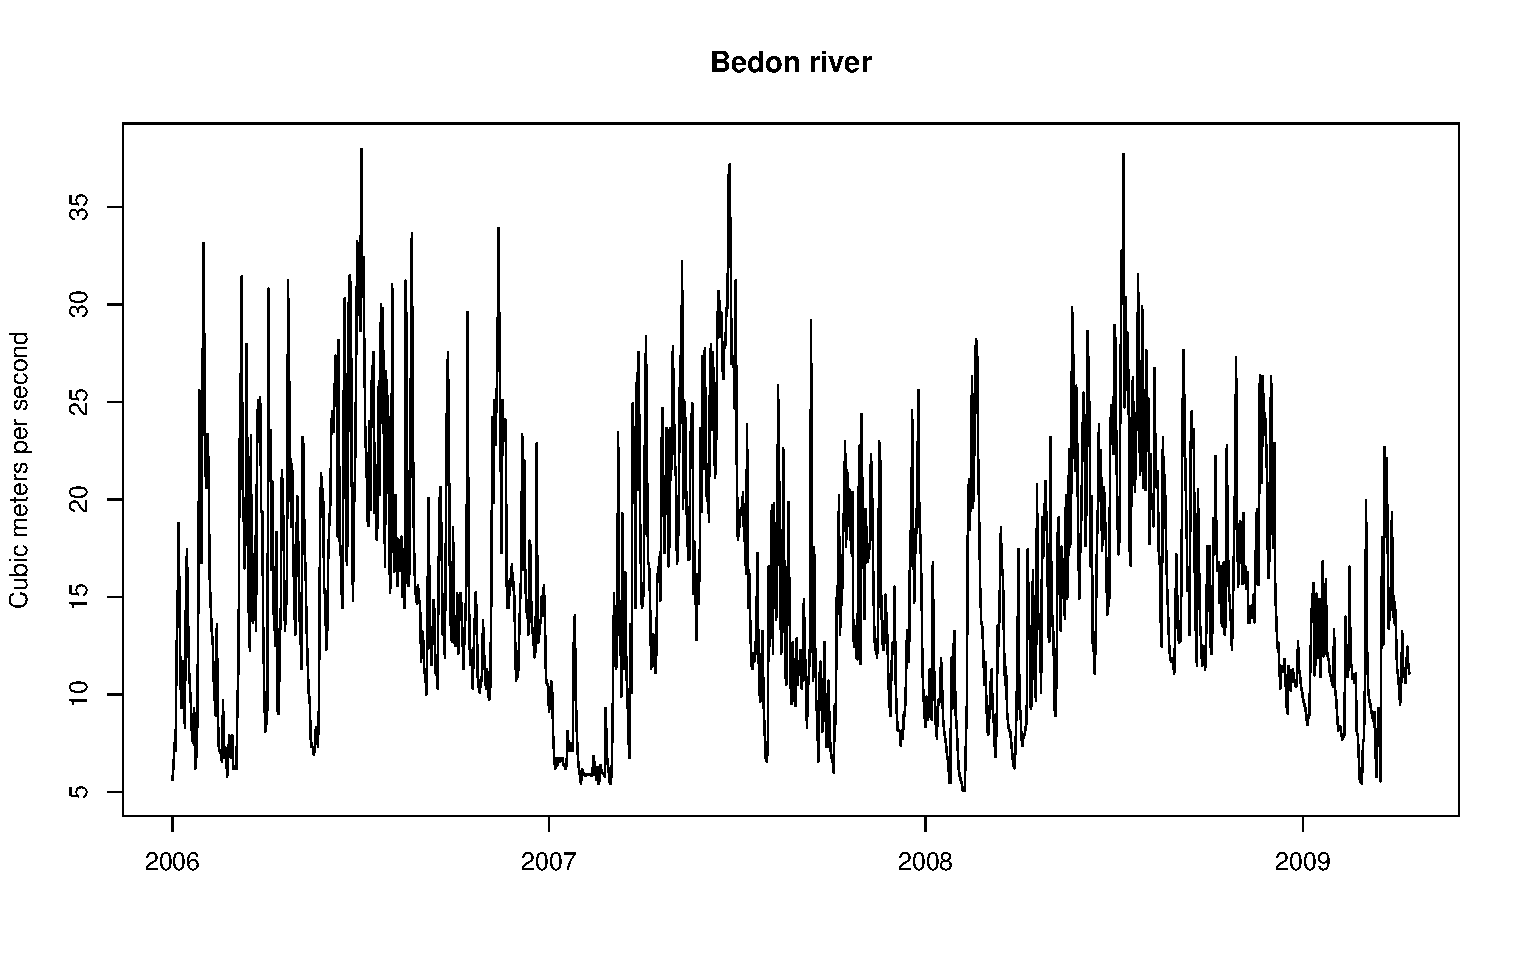
\includegraphics[width=11cm]{figures/Bedon1}\\
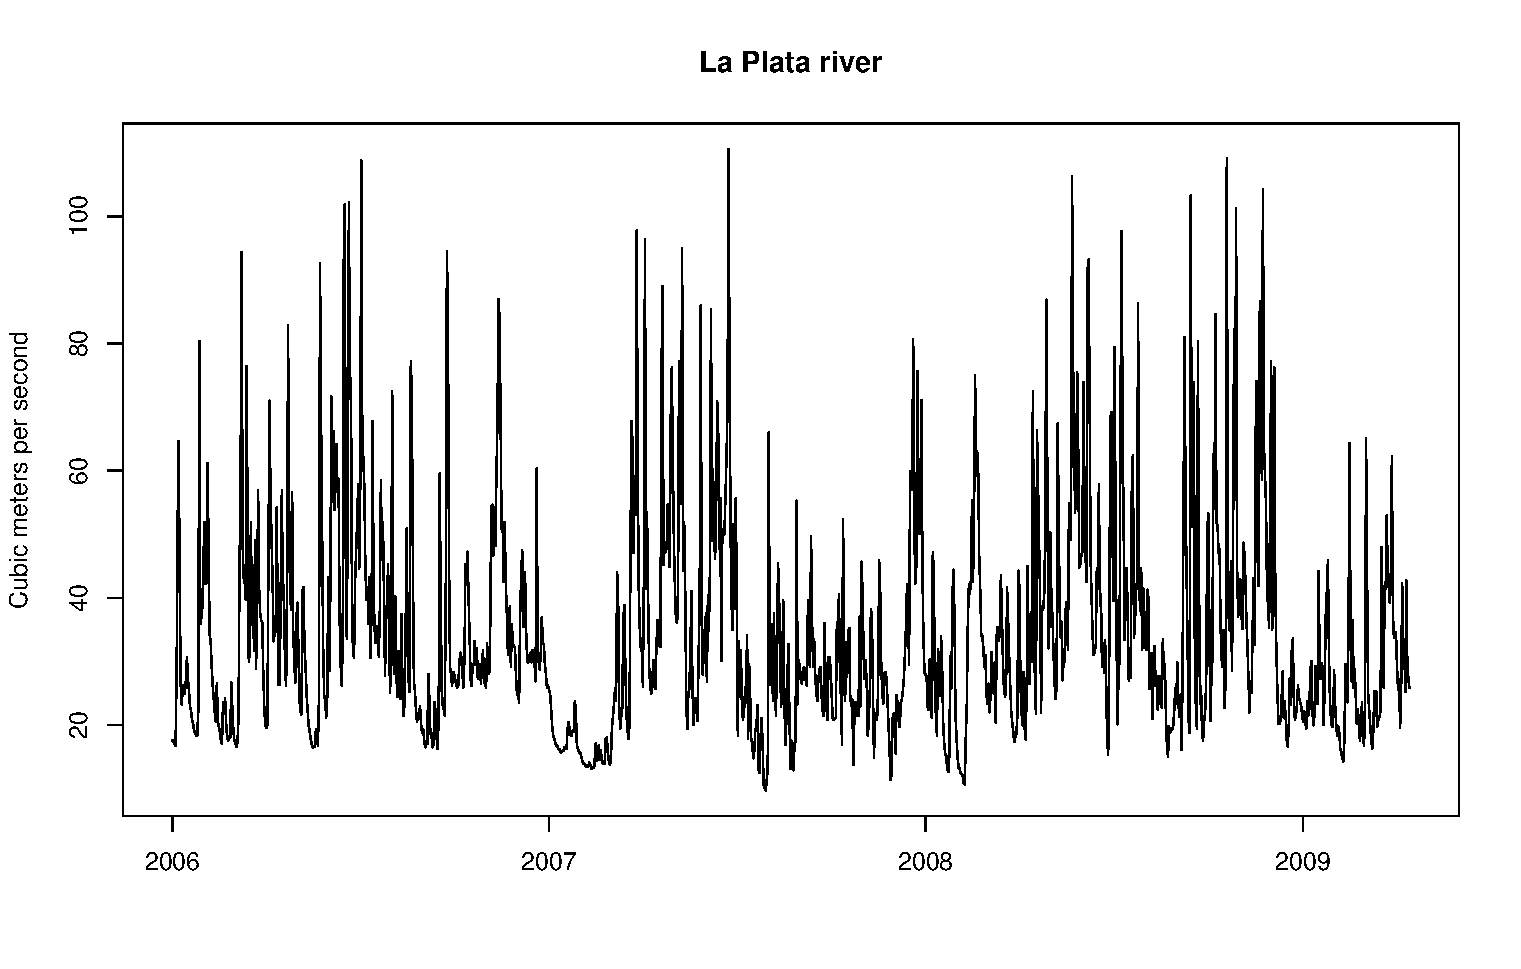
\includegraphics[width=11cm]{figures/LaPlata1}
\caption{Time series plots of rainfall (a), Bedon River flow (b), and La Plata River flow (c).}
\label{inputYout}
\end{figure}

\begin{table}[!ht]
{\small
\begin{center}
\begin{tabular}{lll} 
 \hline
Column &  Role &  Description\\ \hline
\code{Date}     & Labels for time points & Dates when measurements were taken\\
\code{Rainfall} & Threshold series                               & Rainfall, in $mm$\\
\code{Bedon}    & First component of the output series  & Bedon river flow, in $m^3\!/\!s$\\
\code{LaPlata}  & Second component of the output series & La Plata river flow, in $m^3\!/\!s$\\ 
 \hline
\end{tabular}
\end{center}
\caption{Description of the variables in the \code{riverflows} dataset included in the \CRANpkg{mtarm} package.}
\label{td}}
\end{table}

Figure~\ref{inputYout} displays the three time series described above. A clear association can be observed between rainfall and river flows: periods of elevated precipitation tend to coincide with increased river discharge, particularly in the Bedon River, whereas periods of low rainfall are generally associated with reduced flow levels. This relationship appears less pronounced for the La Plata River, suggesting that the hydrological response to precipitation may differ between the two river systems. Overall, these patterns indicate a strong dependence of river discharge on rainfall and suggest that the underlying dynamics may vary across hydrological conditions. Such behavior is consistent with the presence of threshold effects in the river-flow dynamics. In particular, the relationship between rainfall and river discharge may change when precipitation exceeds or falls below certain critical levels, giving rise to distinct dynamic regimes. This possibility motivates the use of a regime-switching framework. The multivariate TAR model is especially well suited to this setting, as it allows the joint dynamics of the Bedon and La Plata river flows to evolve differently across rainfall regimes. To reproduce this exploratory analysis, the following code can be used to generate the corresponding plots:

\begin{example}
> data(riverflows)
> str(riverflows)
Classes ‘tbl_df’, ‘tbl’ and 'data.frame':   1200 obs. of  4 variables:
 $ Date    : Date, format: "2006-01-01" "2006-01-02" ...
 $ Bedon   : num  5.6 6.36 7.5 7.11 12.39 ...
 $ LaPlata : num  17.6 17.3 17.1 16.8 28.5 ...
 $ Rainfall: num  0 0 0 4 0 ...
>
> dev.new()
> par(mfrow=c(3,1))
> with(riverflows,{plot(Date, Rainfall, type="l", lty=1, col="black", xlab="", 
+                       ylab="Millimeters", main="Rainfall")
+                  plot(Date, Bedon, type="l", lty=1, col="black", xlab="", 
+                       ylab="Cubic meters per second", main="Bedon river")
+                  plot(Date, LaPlata, type="l", lty=1, col="black", xlab="", 
+                       ylab="Cubic meters per second", main="La Plata river")})
\end{example}

\subsection{Fitting a TAR model}
\begin{example}
> args(mtar)
function(formula, data, subset, Intercept=TRUE, trend=c("none","linear","quad"), 
         nseason=NULL, ars=ars(), row.names, dist=dist=c("Gaussian","Student-t",
         "Hyperbolic","Laplace","Slash","Contaminated normal","Skew-Student-t",
         "Skew-normal"), prior=list(), n.sim=500, n.burnin=100, n.thin=1, 
         ssvs=FALSE, setar=NULL, progress=TRUE, ...)
\end{example}
The routine \code{mtar()} performs Bayesian estimation in multivariate TAR models, including SETAR and VAR models, and their univariate versions, as described by \cite{VANEGAS2025}. In that routine, the user can specify several features of both the TAR model to be fitted to the data and the MCMC algorithm to be used to draw a sample from the posterior distribution of the model parameters. Some of those features are the following: $(i)$ components of the model, that is, the output time series, the threshold time series, and the exogenous time series; $(ii)$ number of regimes; $(iii)$ the autoregressive order for $\{\bm{Y}_t\}_{_{t\geq 1}}$ and the maximum lags for $\{\bm{X}_t\}_{_{t\geq 1}}$ and $\{Z_t\}_{_{t\geq 1}}$ within each regime; $(iv)$ noise process distribution; $(v)$ hyperparameter values; and $(vi)$ chain size, thinning interval and burn-in period for the MCMC algorithm. The main arguments in the routine \code{mtar()} are the following:

\begin{itemize}
\item \underline{\bf formula}. This Formula-type argument allows us to specify the output time series, the threshold time series (if any), and the exogenous time series (if any). Formula-type objects provided by the package \code{Formula} (\citet{ZC10}) extend the base class \code{formula} by allowing for multiple responses and multiple parts of regressors. For example, \code{formula = $\sim$ y1 + y2 + y3 | z | x1 + x2} indicates the following: $(i)$ the output time series, $\{\bm{Y}_t\}_{_{t\geq 1}}$, is tridimensional and its realization is composed of the columns named \code{y1}, \code{y2} and \code{y3}; $(ii)$ the realization of the threshold time series, $\{Z_t\}_{_{t\geq 1}}$, is the column named \code{z}; and $(iii)$ the exogenous time series, $\{\bm{X}_t\}_{_{t\geq 1}}$, is bidimensional and its realization is composed of the columns named \code{x1} and \code{x2}. The columns named \code{y1}, \code{y2}, \code{y3}, \code{z}, \code{x1} and \code{x2} are assumed to be included in the data.frame specified in the argument \code{data} in the call to the routine \code{mtar()}. Indeed, if the data.frame-type object specified in the argument \code{data} contains only the variables comprising the output time series, a \code{VAR(p)} model can be specified by \code{formula\,\,=\,\,}$\sim .$

\item \underline{\bf ars}. This list-type argument allows us to specify values for $l$ (number of regimes), $\bm{p}=(p_1,\ldots,p_l)$, $\bm{q}=(q_1,\ldots,q_l)$ and $\bm{d}=(d_1,\ldots,d_l)$. The helper function {\tt ars()} simplifies the model setup specification in \code{ars}. For example, \code{ars(nregim=3,p=2)} sets a TAR model with 3 regimes and an autoregressive order of 2 within each regime. Similarly, \code{ars(nregim=3,p=2,q=3)} sets a TAR model with 3 regimes, an autoregressive order of 2 within each regime, and a maximum lag of 3 for the exogenous time series within each regime. Moreover, \code{ars(nregim=3, p=c(1,2,1),\tt q=c(2,} \code{0,3), d=c(1,1))} indicates the following: $(i)$ the number of regimes is $3$; $(ii)$ the autoregressive order in the first, second and third regimes is $1$, $2$ and $1$, respectively; $(iii)$ the maximum lag for the exogenous time series in the first, second and third regimes is $2$, $0$ and $3$, respectively; $(iv)$ the maximum lag for the threshold time series in the first, second and third regimes is $1$, $1$ and $0$, respectively.  The inclusion of \code{p} in  \code{ars()} is mandatory, whereas \code{q} and \code{d} are optional. Indeed, when a threshold series is specified in the argument \code{formula}, the inclusion of \code{d} becomes relevant, but it is not necessary. In addition, if \code{q}/\code{d} is missing, then \code{ars()} assumes that the maximum lag for the exogenous/threshold series is $0$ in all regimes.

\item \underline{\bf data}. A data.frame-type object with rows representing time points, arranged ascendingly according to the time and containing at least the following columns: $(i)$ all those used to specify the TAR model in the argument \code{formula}, that is, those composing the output time series, the threshold time series (if any), and the exogenous time series (if any); $(ii)$ that specified in the optional argument \code{row.names} to label the time points; $(iii)$ those utilized in the optional argument \code{subset} to choose a subset of the rows of the data.frame to be used in the fitting process. If the argument \code{data} is missing, then the columns are taken from \code{environment(formula)}, typically the environment from which the routine \code{mtar()} is called.

\item \underline{\bf Intercept}. This logical-type argument allows us to specify whether there are intercept terms in the model, that is, if there are $\phi_0^{^{(j)}}\neq 0$ for $j=1,\ldots,l$. By default, \code{Intercept} is set to \code{TRUE}.

\item \underline{\bf trend}. This character string allows users to specify the degree of a deterministic time trend to be included in each regime. The available options are: linear trend (``linear''), quadratic trend (``quadratic''), and no time trend (``none''). By default, \code{trend} is set to ``none''.

\item \underline{\bf nseason}. This integer value allows us to specify the number of seasonal periods. If \code{nseason} is specified then \code{nseason}-1 seasonal dummies are added to the regressors within each regime. As described in section \ref{mf}, those seasonal dummies are obtained by vertically stacking several \code{nseason}$\times$ \code{nseason} identity matrices with their first column removed.

\item \underline{\bf dist}. A character-type argument that allows us to specify a multivariate distribution to describe the noise process behavior. Available options are: Gaussian ({\tt``Gaussian''}), Student-$t$ ({\tt``Student-t''}), Slash (\code{``Slash''}), symmetric Hyperbolic (\code{``Hyperbolic''}), contaminated normal (\code{``Contaminated normal''}), Laplace (\code{``Laplace''}), skew-normal (\code{``Skew-normal''}) and Skew-$t$ (\code{``Skew-Student-t''}). By default, \code{dist} is set to \code{``Gaussian''}. 

\item \underline{\bf prior}. A list-type argument that allows us to specify the hyperparameter values described in section \ref{pd}. By default, they are set to the following values, which ensure non-informative prior distributions: $h_{\rm min}=0$, $h_{\rm max}=3$, $\alpha_0=0$, $\alpha_1=1$, $\omega_0=10^{-9}$, $\tau_0=k$, $\mu_0=0$, $\delta_0=10^9$, $\rho_0=0.5$, $\lambda_0=10^9$, and
\begin{itemize}
\item for the Student-$t$ and skew-$t$ cases, $\gamma_{0}=1$ and $\eta_{0}=100$;
\item for the Slash case, $\gamma_{0}=10^{-9}$ and $\eta_{0}=10^{-9}$;
\item for the contaminated normal case, $\gamma_{01}=10^{-9}$, $\eta_{01}=10^{-9}$, $\gamma_{02}=10^{-9}$ and $\eta_{02}=10^{-9}$; 
\item for the symmetric hyperbolic case, $\gamma_{0}=0.1$ and $\eta_{0}=4$.
\end{itemize} 
For example, \code{prior=list(hmin=0,hmax=3,theta0=0,delta0=1e+09,omega0=1e-09,tau0=k)} indicates that $h_{\rm min}$, $h_{\rm max}$, $\theta_0$, $\delta_0$, $\omega_0$ and $\tau_0$ are set to $0$, $3$, $0$, $10^9$, $10^{-9}$ and $k$, respectively, while the other hyperparameters are set to their default values. Similarly, \code{prior=list(hmax=5)} indicates that $h_{\rm max}$ is set to $5$, whereas the other hyperparameters are set to their default values. Finally, \code{prior=list(hmin=3,hmax=3)} indicates that the delay parameter $h$ is known and equal to $3$. The routine \code{mtar()} uses the helper function {\tt priors()} to validate the argument \code{prior}. Practical guidance on selecting the hyperparameters that determine the bounds of the delay and threshold parameters has been added to Appendix~\ref{priors}.

\item \underline{\bf n.burnin, n.sim, n.thin}. These integer-type arguments allow us to specify the number of iterations that the MCMC-type algorithm must perform, where \code{n.sim}, \code{n.thin} and \code{n.burnin} represent, respectively, the chain size, the thinning interval, and the length of the burn-in period. Hence, the MCMC-type algorithm performs \code{n.burnin}\,\, + \,\,\code{n.sim}\,$\times$\,\code{n.thin} iterations, from which \code{n.sim} iterations are returned, so that \code{n.burnin}\,\, + \,\,\code{n.sim}\,$\times$\,(\code{n.thin}\,\,-\,\,1) are discarded. The \code{n.sim} iterations that the routine \code{mtar()} returns correspond to those at the following positions:

\begin{center}
\begin{tabular}{c|l}
1  & \code{n.burnin}\,\,+\,\,1,\\
2 &\code{n.burnin}\,\,+\,\,1\,\,+\,\,(1\,$\times$\,\code{n.thin}),\\
3  &\code{n.burnin}\,\,+\,\,1\,\,+\,\,(2\,$\times$\,\code{n.thin}),\\
\vdots   & \vdots\\
\code{n.sim}  &\code{n.burnin}\,\,+\,\,1\,\,+\,\,((\code{n.sim}\,\,-\,\,1)\,$\times$\,\code{n.thin}).
\end{tabular}
\end{center}

\item \underline{\bf ssvs}. If \code{ssvs=TRUE} is specified, then the Stochastic Search Variable Selection (SSVS) procedure is applied to identify relevant lags of the output, exogenous (if any), and threshold (if any) series. As a consequence, the components of $\bm{\zeta}_1,\ldots,\bm{\zeta}_l$ are estimated as part of the MCMC-type algorithm. The length and structure of each $\bm{\zeta}_j$ depends on the argument \code{ars}. Specifically, for $j=1,...,l$, $\bm{\zeta}_j$ is a vector combining three blocks: $(\zeta_{j,1},...,\zeta_{j,p_j})$, $(\zeta_{j,p_j+1},...,\zeta_{j,p_j+q_j})$, and $(\zeta_{j,p_j+q_j+1},\ldots,\zeta_{j,p_j+q_j+d_j})$, so that $\bm{\zeta}_j = (\zeta_{j,1},...,\zeta_{j,p_j}, \zeta_{j,p_j+1},...,\zeta_{j,p_j+q_j}, \zeta_{j,p_j+q_j+1},...,\zeta_{j,p_j+q_j+d_j})$. If \code{ssvs=FALSE} then $\bm{\zeta}_1,\dots,\bm{\zeta}_l$ are assumed to be known and set to vectors of ones. By default, \code{ssvs} is set to \code{FALSE}.

\item \underline{\bf setar}. If \code{setar = m} is specified, a SETAR model is fitted, where \code{m} identifies the component of the multivariate time series used as the threshold variable. In this case, the hyperparameter $h_{\rm min}$ is automatically set to \code{1} (instead of its default value, \code{0}), since the delay parameter in a SETAR model must be positive. By default, \code{setar = NULL}, indicating that a general TAR model, rather than a SETAR model, is fitted.

\item \underline{\bf progress}. If \code{progress=TRUE} is specified, then a progress bar is displayed during the execution of the MCMC-type algorithm. By default, \code{progress} is set to \code{TRUE}.

\end{itemize}

To demonstrate the use of this routine, we fit a bivariate $\text{TAR}(2; p=(5,5), d=(5,5))$ model to the original data, following the specification considered by \cite{CN17}. As a linear benchmark, we also estimate a standard $\text{VAR}(5)$ model with Gaussian innovations. In the TAR specification, rainfall serves both as the threshold variable and as an exogenous predictor. A notable feature of this analysis is the use of the Stochastic Search Variable Selection (SSVS) procedure implemented in \code{mtar()}, which enables automatic identification of the relevant lag structures within the Bayesian estimation framework. Although SSVS methods are available for linear models in packages such as \code{bvartools}, extending Bayesian lag selection to multivariate threshold autoregressive models constitutes an important feature of \CRANpkg{mtarm}. For the empirical analysis, observations from January 1, 2006, to April 4, 2009, are used for model estimation, while the final 10 observations are reserved for out-of-sample forecast evaluation. Posterior inference is based on an MCMC algorithm with 9000 iterations. The first 3000 iterations are discarded as burn-in, and a thinning factor of 2 is applied to the remaining draws, resulting in a posterior sample of 3000 observations. The models can be estimated using the following code:

\begin{example}
> set.seed(2000)
> model_TAR <- mtar(~ Bedon + LaPlata | Rainfall, row.names=Date, dist="Gaussian", 
+                   data=riverflows, subset={Date<="2009-04-04"}, ssvs=TRUE,
+                   ars=ars(nregim=2,p=5,d=5), n.burnin=3000, n.sim=3000, n.thin=2)
> model_VAR <- update(model_TAR, ars=ars(nregim=1,p=5))
\end{example}

The \code{mtar()} function returns an object of class \code{mtar}, for which a range of standard methods are available, including \code{print()}, \code{summary()}, \code{coef()}, \code{vcov()}, \code{model.matrix()}, \code{fitted()}, \code{plot()}, \code{predict()}, and \code{residuals()}. In addition, fitted models can be compared using model assessment criteria such as the Deviance Information Criterion (DIC) \citep{spiegelhalter02,spiegelhalter14} and the Watanabe--Akaike Information Criterion (WAIC) \citep{w10}, which are implemented in \CRANpkg{mtarm} through the functions \code{DIC()} and \code{WAIC()}, respectively. To compare the in-sample performance of the fitted models and assess whether the additional flexibility of the nonlinear specification is supported by the data, we compute the DIC and WAIC for both estimated models as follows:

\begin{example}
> DIC(model_TAR, model_VAR)
                DIC
model_TAR  14186.12
model_VAR  15654.09
>
> WAIC(model_TAR, model_VAR)
               WAIC
model_TAR  14369.19
model_VAR  15793.80
\end{example}

Both information criteria favor the TAR specification (\code{model\_MTAR}) over the linear benchmark (\code{model\_VAR}), as indicated by the lower DIC and WAIC values obtained for the former model. This result suggests that the additional flexibility introduced by the threshold structure is supported by the observed data and leads to an improved in-sample fit. From a modeling perspective, these findings provide evidence that allowing the dynamics to vary across rainfall regimes captures important features of the river-flow processes that are not adequately represented by a conventional linear VAR model. Consequently, the results support the use of a threshold autoregressive framework for describing the nonlinear relationship between rainfall and river discharge in this application.

\subsection{Residual analysis}
Next, we examine the residuals of the fitted multivariate TAR model to assess the adequacy of the Gaussian innovation assumption. Specifically, we compute the quantile-type residuals \citep{dunn1996randomized}, including the joint residuals $r_t^{^{\!(2)}}$ for $t=1,\ldots,T$ and the componentwise residuals $r_{m,t}^{^{\!(1)}}$ for $m=1,2$ and $t=1,\ldots,T$. These residuals are obtained using the following code and stored in the list object \code{res}. The element \code{full} contains the joint residuals $r_t^{^{\!(2)}}$, whereas \code{by.component} stores the componentwise residuals $r_{m,t}^{^{\!(1)}}$. The residual diagnostics can then be performed as follows:

\begin{example}
> set.seed(0202)
> res_model_TAR <- residuals(model_TAR)
> plot(res_model_TAR, col="blue")
\end{example}

Figure~\ref{Resdiagnostic} displays the normal Q-Q plot and histogram of the quantile-type residuals. Since quantile-type residuals are expected to behave as a random sample from the standard normal distribution when the fitted model is correctly specified, these results provide additional evidence supporting the
adequacy of the selected models. The diagnostic plots indicate noticeable departures from normality, particularly in the tails of the distribution, where several extreme observations are apparent. Such patterns suggest that the Gaussian innovation assumption may not adequately describe the residual behavior and motivate the consideration of more flexible distributions, such as the Student-$t$, Laplace, or skew-$t$ families. The residual diagnostics are readily obtained through the tools implemented in \CRANpkg{mtarm}, which facilitate the computation and extraction of quantile-type residuals for multivariate TAR models. These diagnostics provide a useful basis for evaluating distributional assumptions and guiding the selection of alternative innovation distributions when warranted by the data.

\begin{figure}
\centering
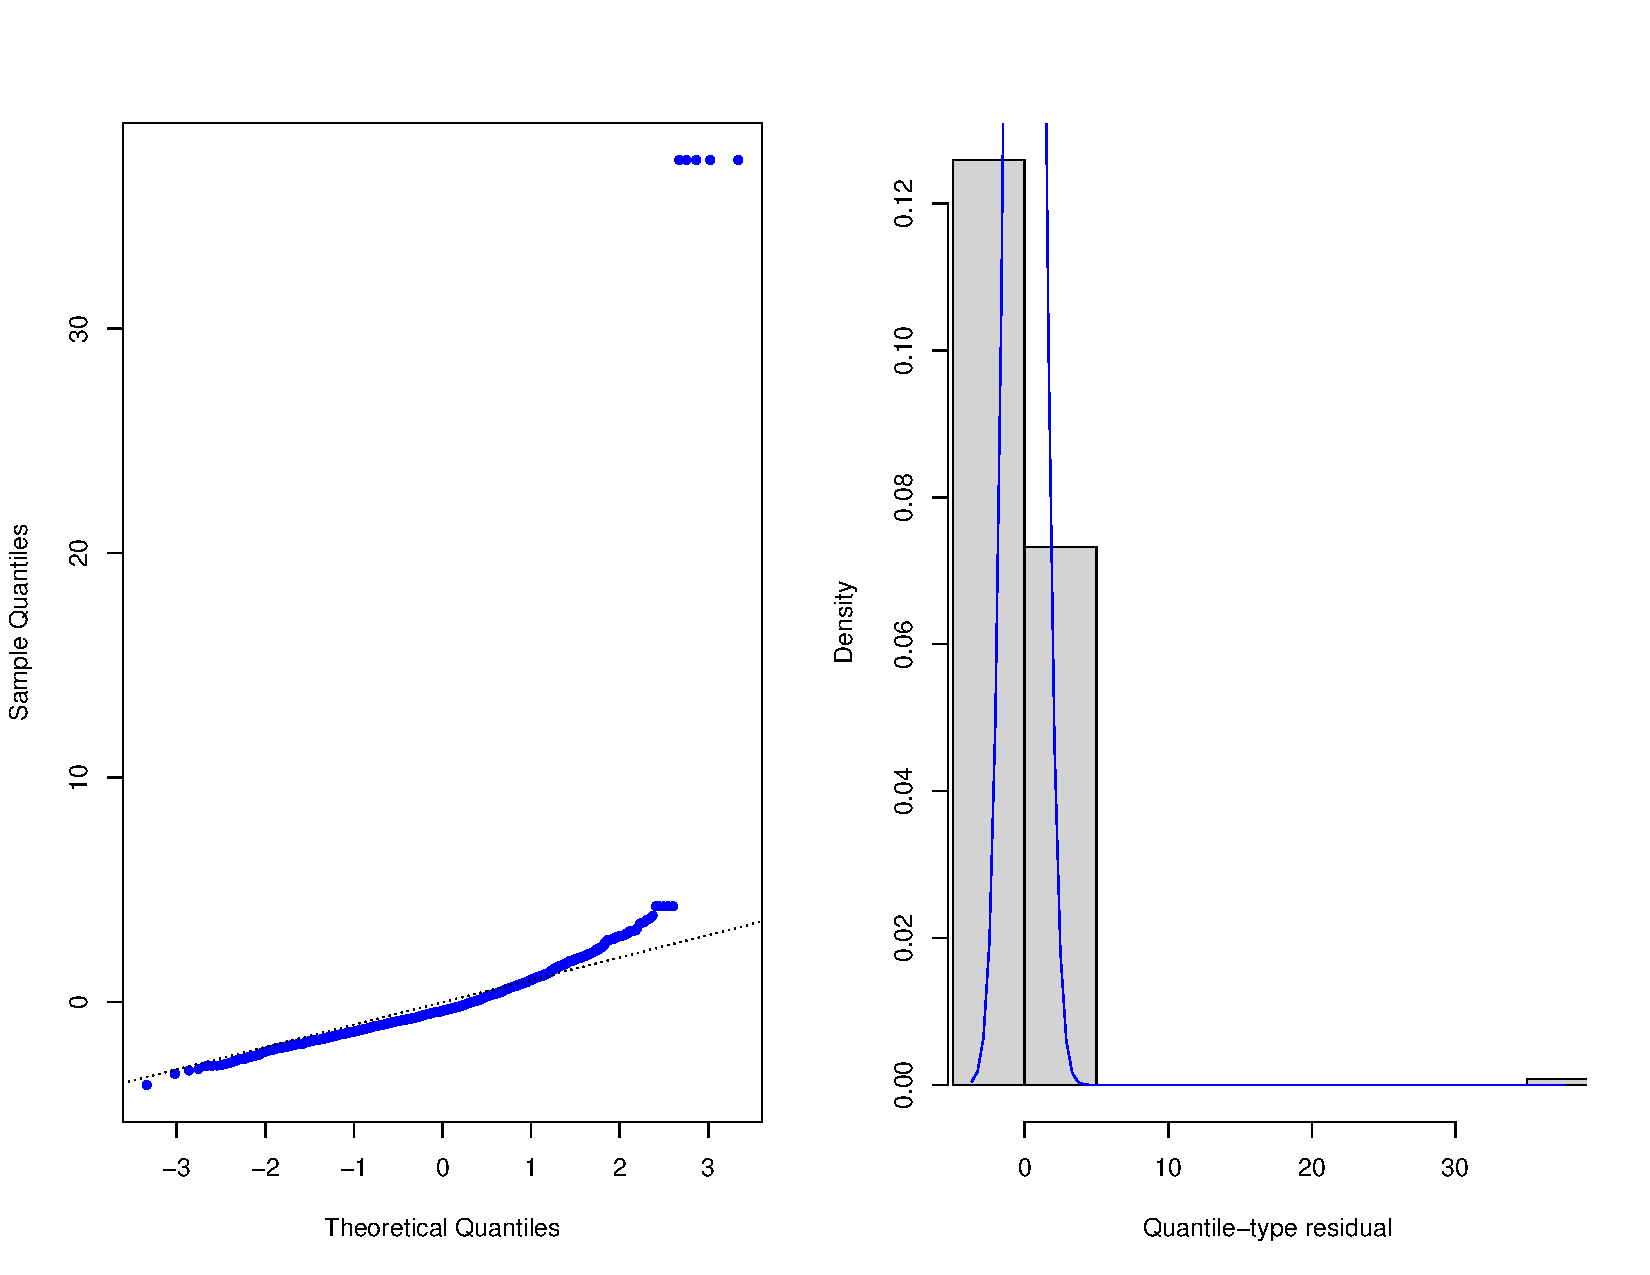
\includegraphics[scale=0.4]{figures/Diagnostic_MTAR_Gauss_Riv_col}
\caption{Diagnostic plots of the quantile-type residuals for the ${\rm TAR}(2;\bm{p}=(5,5))$ model with Gaussian innovations: Normal Q-Q plot (a) and histogram (b).}

\label{Resdiagnostic}
\end{figure}

To systematically explore candidate models with different innovation distributions, numbers of regimes, and lag structures, \CRANpkg{mtarm} provides the function \code{mtar\_grid()}. This routine serves as a wrapper around \code{mtar()}, automatically fitting a collection of models defined over a user-specified grid of configurations. In particular, it evaluates combinations of: $(i)$ the innovation distribution specified through \code{dist}; $(ii)$ the number of regimes, ranging from \code{nregim.min} to \code{nregim.max}; $(iii)$ the autoregressive order within each regime, ranging from \code{p.min} to \code{p.max}; $(iv)$ the maximum lag of the exogenous series, ranging from \code{q.min} to \code{q.max}; and $(v)$ the maximum lag of the threshold series, ranging from \code{d.min} to \code{d.max}. The arguments \code{dist}, \code{nregim.min}, \code{nregim.max}, \code{p.min}, \code{p.max}, \code{q.min}, \code{q.max}, \code{d.min}, and \code{d.max} therefore define the model search space explored by \code{mtar\_grid()}. The function returns a list whose elements are objects of class \code{mtar}, each corresponding to a distinct model specification. This facilitates systematic model comparison and selection within a unified framework. As with any flexible threshold autoregressive model, increasing the number of regimes improves model flexibility but also increases the number of parameters to be estimated. Consequently, regimes containing relatively few observations may lead to weakly identified parameters and greater posterior uncertainty. In practice, potential identifiability issues can be investigated using the convergence diagnostics available in \CRANpkg{mtarm}, such as Geweke's diagnostic and effective sample size, together with posterior summaries including High Posterior Density (HPD) intervals. Unusually wide HPD intervals may indicate that a model is overly complex relative to the information available in the data. Users should also be aware of the computational trade-offs associated with richer model specifications. In particular, heavy-tailed innovation distributions typically require the introduction of latent variables within the MCMC algorithm, increasing computational cost per iteration. A practical strategy is to conduct an initial grid search using relatively short MCMC runs to eliminate clearly inferior specifications before refitting a smaller set of promising candidates using longer chains.
In addition, fitted models can be compared using out-of-sample predictive performance measures, including the Absolute Error (AE), Absolute Percentage Error (APE), Squared Error (SE), log-score \citep{Good1952}, Energy Score \citep{GneitingEtAl2008TEST}—a multivariate generalization of the Continuous Ranked Probability Score (CRPS) \citep{MathesonWinkler1976,GrimitGneitingBerrocalJohnson2006}—, and other forecasting metrics available through the \code{out\_of\_sample()} function. Finally, the \code{plan\_strategy} argument of \code{mtar\_grid()} enables parallel computation through the packages \CRANpkg{future} \citep{future} and \CRANpkg{future.apply} \citep{future.apply}, substantially reducing computation times when a large number of candidate models are considered.

\subsection{Improving the fit: exploration of alternative models}
To improve model fit and assess the impact of model complexity, a total of 20 candidate models are fitted to the data. Specifically, we consider the families ${\rm VAR}(p^*)$, ${\rm TAR}(2;\bm{p}=(p^*,p^*))$, ${\rm TAR}(3;\bm{p}=(p^*,p^*,p^*))$, and ${\rm TAR}(4;\bm{p}=(p^*,p^*,p^*,p^*))$, with $p^*=1,\ldots,5$. This model set allows us to jointly evaluate the effects of autoregressive order and the number of regimes on predictive performance and goodness of fit. To accommodate the outliers identified in the residual diagnostics, the innovation process $\bm{\epsilon}_{t_j}$ is assumed to follow a multivariate Laplace distribution. This heavy-tailed specification provides increased robustness to extreme observations and departures from normality. More generally, one of the key strengths of \CRANpkg{mtarm} is its ability to estimate multivariate TAR models under a broad range of non-Gaussian innovation distributions, thereby extending the scope of existing software for threshold autoregressive modeling in \code{R}. The candidate models considered in this analysis can be expressed as follows:
$$\bm{Y}_t=\sum\limits_{j=1}^{l} I(Z_{t-h}\in(c_{j-1},c_j])\!\Big(\!\bm{\phi}_0^{^{(j)}}+\sum\limits_{i=1}^{p^*}\bm{\phi}_i^{^{(j)}}\bm{Y}_{t-i}+\bm{\epsilon}_{t_j}\!\Big),$$
where $\bm{\epsilon}_{t_j} \myeq \text{Laplace}(\bm{0},\bm{\Sigma}_j)$. 
Meaningful comparisons across fitted models require that all models be estimated using the same effective sample period. In autoregressive settings, however, the first $m$ observations of the observed series cannot be used for estimation because they are needed to construct the lagged predictors. Consequently, the effective sample size is $T-m$, where $T$ denotes the length of the observed series. For $\text{VAR}(p^*)$ models (i.e., a single-regime specification), $m=p^*$. For threshold autoregressive models with two or more regimes, the effective sample offset is given by $m = \text{max}(p^*, h_{\rm max})$, where $h_{\max}$ denotes the upper bound of the prior support for the delay parameter $h$, whose default value in \CRANpkg{mtarm} is 3. The \code{mtar\_grid()} function automatically adjusts the effective sample period for each fitted model, ensuring that all model comparisons are based on the same set of observations.

\subsubsection{Model estimation}
The following code uses the wrapper function \code{mtar\_grid()} to systematically fit a collection of candidate models by repeatedly calling \code{mtar()} over all combinations of the number of regimes ($l=1,\ldots,4$) and autoregressive orders ($p^*=1,\ldots,5$). The resulting fitted models are stored in the list object \code{models}, whose elements are named \code{Laplace.}$l.p^*$, corresponding to the model with $l$ regimes and autoregressive order $p^*$.
For each candidate model, \code{mtar()} is configured as follows: $(i)$ relevant lagged effects of $\{\bm{Y}_t\}_{t\geq 1}$ are identified separately within each regime using the Stochastic Search Variable Selection (SSVS) procedure (\code{ssvs=TRUE}); $(ii)$ default hyperparameter values are employed, yielding non-informative prior distributions for all model parameters; $(iii)$ posterior inference is based on an MCMC algorithm with 9000 iterations, of which the first 3000 are discarded as burn-in and the remaining draws are thinned by retaining every second sample; $(iv)$ the estimation period spans January 6, 2006, to April 4, 2009; $(v)$ the last ten observations (April 5, 2009, to April 14, 2009) are reserved for out-of-sample forecast evaluation; and $(vi)$ observation dates are provided through the \code{Date} column of the \code{riverflows} data frame. To reduce the overall computation time, \code{mtar\_grid()} is instructed to fit the candidate models in parallel by specifying \code{plan\_strategy = "multisession"}.
\begin{example}
> set.seed(0220)
> models <- mtar_grid(~ Bedon + LaPlata | Rainfall, row.names=Date, dist="Laplace",
                      data=riverflows, subset={Date<="2009-04-04"}, nregim.min=1, 
                      nregim.max=4, p.min=1, p.max=5, n.burnin=3000, n.sim=3000, 
                      n.thin=2, ssvs=TRUE, plan_strategy="multisession")
> models

Sample size          : 1185 time points (2006-01-06 to 2009-04-04)
Output Series        : Bedon    |    LaPlata
Threshold Series     : Rainfall
Error Distribution   : Laplace
Number of regimes    : 1 to 4
Deterministics       : Intercept  
Autoregressive orders: 1 to 5
\end{example}

\subsubsection{Model selection}
The fitted models are then compared using adjusted within-sample predictive accuracy measures, such as DIC and WAIC. According to the following code, a first matrix, named \code{DICs}, stores the values of the DIC criterion for the twenty fitted models, whereas a second matrix, named \code{WAICs}, stores the values of the WAIC criterion for the twenty fitted models. In both cases, the rows represent the different values of $p^*$, whereas the columns represent the different values of the number of regimes $l$.

\begin{example}
> DICs <- matrix(DIC(models),5,4)
> rownames(DICs) <- paste0("p*=",1:5)
> colnames(DICs) <- c("VAR(p*)","TAR(2;p*,p*)","TAR(3;p*,p*,p*)","TAR(4;p*,p*,p*,p*)")
> round(DICs,2)
      VAR(p*) TAR(2;p*,p*) TAR(3;p*,p*,p*) TAR(4;p*,p*,p*,p*)
p*=1 14490.90     13757.46        13573.22           13500.45
p*=2 14423.63     13726.43        13572.99           13519.93
p*=3 14422.83     13681.53        13568.18           13458.78
p*=4 14421.12     13680.52        13525.78           13447.31
p*=5 14385.23     13637.01        13504.93           13433.73
>
> WAICs <- matrix(WAIC(models),5,4)
> rownames(WAICs) <- rownames(DICs)
> colnames(WAICs) <- colnames(DICs)
> round(WAICs,2)
      VAR(p*) TAR(2;p*,p*) TAR(3;p*,p*,p*) TAR(4;p*,p*,p*,p*)
p*=1 14494.80     13765.46        13585.76           13540.82
p*=2 14428.96     13737.65        13587.31           13545.79
p*=3 14429.75     13695.53        13591.64           13479.35
p*=4 14429.73     13694.27        13564.89           13482.35
p*=5 14391.72     13737.57        13531.97           13499.51
\end{example}
Compared with linear specifications (i.e., VAR models), nonlinear alternatives, namely TAR models with two, three, and four regimes, exhibit superior performance under both criteria. For a fixed autoregressive order $p^*$, models with four regimes consistently yield the lowest DIC and WAIC values, whereas single-regime models perform worst. Likewise, for a fixed number of regimes $l$, models of order 5 generally attain the lowest DIC and WAIC values, while order 1 models tend to have the highest. According to the DIC, the preferred specification is ${\rm TAR}(3;\bm{p}=(3,3,3))$, whereas the WAIC favors ${\rm TAR}(4;\bm{p}=(3,3,3,3))$. To complement the in-sample model assessment, several out-of-sample predictive accuracy measures are also evaluated. Specifically, we consider the average log-score (LS), the average Energy Score (ES) and the Mean Absolute Percentage Error (MAPE) for each component of the multivariate response series. The following code computes these measures using the hold-out observations reserved for forecast evaluation. The resulting values are then aggregated using the function supplied through the \code{FUN} argument, which by default is set to \code{mean()}. This allows users to summarize predictive performance according to alternative criteria if desired. The resulting values are stored in the matrices \code{LSs}, \code{ESs}, \code{APE.1s}, and \code{APE.2s}. In each matrix, rows correspond to different autoregressive orders $p^*$, whereas columns correspond to different numbers of regimes $l$.

\begin{example}
> set.seed(0220)
> future.obs <- subset(riverflows, Date>"2009-04-04")                  
> oos <- out_of_sample(models, newdata=future.obs, n.ahead=nrow(future.obs), FUN=mean)
> 
> LSs <- matrix(oos[,1],nrow=5,ncol=4)
> rownames(LSs) <- rownames(DICs)
> colnames(LSs) <- colnames(DICs)
> round(LSs,2)
     VAR(p*) TAR(2;p*,p*) TAR(3;p*,p*,p*) TAR(4;p*,p*,p*,p*)
p*=1    6.27         6.14            5.96               6.02
p*=2    6.21         6.02            5.94               5.98
p*=3    6.22         5.99            5.94               5.97
p*=4    6.21         5.98            5.90               5.97
p*=5    6.10         5.98            5.80               5.92
> 
> ESs <- matrix(oos[,2],nrow=5,ncol=4)
> rownames(ESs) <- rownames(DICs)
> colnames(ESs) <- colnames(DICs)
> round(ESs,2)
     VAR(p*) TAR(2;p*,p*) TAR(3;p*,p*,p*) TAR(4;p*,p*,p*,p*)
p*=1   12.56         9.76            8.24               8.46
p*=2   12.45         9.62            8.19               8.40
p*=3   12.44         9.51            8.25               8.15
p*=4   12.43         9.49            8.12               8.13
p*=5   11.80         9.35            7.95               8.10
>
> APEs.1 <- matrix(oos[,5],nrow=5,ncol=4)
> rownames(APEs.1) <- rownames(DICs)
> colnames(APEs.1) <- colnames(DICs)
> round(APEs.1,2)
     VAR(p*) TAR(2;p*,p*) TAR(3;p*,p*,p*) TAR(4;p*,p*,p*,p*)
p*=1   21.76        25.31           24.15              26.41
p*=2   23.16        22.41           23.23              25.97
p*=3   23.29        21.76           23.33              25.07
p*=4   22.33        21.33           22.33              24.85
p*=5   19.98        21.29           20.10              23.52
>
> APEs.2 <- matrix(oos[,6],nrow=5,ncol=4)
> rownames(APEs.2) <- rownames(DICs)
> colnames(APEs.2) <- colnames(DICs)
> round(APEs.2,2)
     VAR(p*) TAR(2;p*,p*) TAR(3;p*,p*,p*) TAR(4;p*,p*,p*,p*)
p*=1   33.61        13.94           11.30              11.06
p*=2   34.59        13.85           11.15              11.27
p*=3   33.91        13.19           11.16              10.28
p*=4   33.60        13.28           11.45              10.46
p*=5   31.75        13.82           11.23              10.56
\end{example}
In contrast to the conclusions suggested by the DIC and WAIC, the out-of-sample predictive measures favor models with three regimes over those with four regimes. For a fixed autoregressive order $p^*$, the three-regime specifications generally achieve the lowest average log-score (LS) and average Energy Score (ES) values, whereas the single-regime model consistently exhibits the weakest predictive performance. Similarly, for a fixed number of regimes $l$, models with $p^*=5$ tend to outperform those with lower autoregressive orders, while models with $p^*=1$ typically perform the worst. Regarding point forecast accuracy, the benefits of introducing TAR-type nonlinearity appear to differ across the two components of the response series. For the Bedon River flow, TAR models with two, three, and four regimes provide only little improvements relative to the corresponding VAR models. For the La Plata River flow, however, the gains are considerably more pronounced, with all TAR specifications substantially outperforming their linear VAR counterparts. Moreover, the average LS, average ES, and MAPE associated with the first response component (the Bedon River flow) consistently identify the ${\rm TAR}(3;\bm{p}=(5,5,5))$ model as the most competitive specification. Taken together, these results suggest that the additional flexibility provided by a three-regime structure yields meaningful gains in predictive performance, while further increasing the number of regimes offers little benefit. This discrepancy between within-sample and out-of-sample criteria illustrates an important practical consideration in time-series modeling. Information criteria such as DIC and WAIC balance model fit and complexity and are computed using the data employed for model estimation. As a result, they may favor more flexible specifications, such as the four-regime model in this application. In contrast, out-of-sample predictive measures evaluate forecasting performance on observations that were not used during estimation and therefore provide a direct assessment of predictive generalization. For practitioners, this example highlights the importance of considering multiple model-selection criteria jointly rather than relying on a single measure. Although the four-regime specification achieved slightly better DIC and WAIC values, the three-regime model consistently outperformed it according to the out-of-sample predictive measures considered. Since forecasting is the primary objective of this application, we selected the three-regime model. More generally, this example illustrates that additional model complexity is not always accompanied by improved predictive performance, and that parsimonious specifications may be preferable when they provide comparable fit while yielding superior forecasts. Consequently, the ${\rm TAR}(3;\bm{p}=(5,5,5))$ model is selected as the preferred specification for subsequent analysis.

\subsubsection{Overview of the chosen model}
The following code requests a summary of the fitted ${\rm TAR}(3;\bm{p}=(5,5,5))$ Laplace model, where the argument \code{credible}, which by default is set to $0.95$, allows the user to specify the required level for the credible intervals of the model parameters.

\begin{example}
> summary(models[["Laplace.3.5"]], credible=0.95)

Sample size          : 1185 time points (2006-01-06 to 2009-04-04)
Output Series (OS)   : Bedon    |    LaPlata
Threshold Series     : Rainfall with a estimated delay equal to 0
Error Distribution   : Laplace
Number of regimes    : 3
Deterministics       : Intercept  
Autoregressive orders: 5 in each regime

Thresholds (Mean, HDI_low, HDI_high)
Regime 1     (-Inf,3.4337]     (-Inf,3.08834]     (-Inf,3.98057]
Regime 2 (3.4337,10.00928] (3.08834,10.00268] (3.98057,10.01671]
Regime 3    (10.00928,Inf)     (10.00268,Inf)     (10.01671,Inf)

Regime1:
     OS.lag(1) OS.lag(2) OS.lag(3) OS.lag(4) OS.lag(5)
SSVS         1         0         0         0         1

Autoregressive coefficients
                  Mean  2(1-PD) HDI.Lower HDI.Upper     Mean  2(1-PD) HDI.Lower HDI.Upper
(Intercept)     1.28929 0.00001  1.08328  1.51231  |  3.59625 0.00001  2.91502  4.30655
Bedon.lag(1)    0.63936 0.00001  0.58745  0.69628  |  0.09655 0.17600 -0.05574  0.22998
LaPlata.lag(1)  0.02471 0.02600  0.00255  0.04455  |  0.61940 0.00001  0.55499  0.68540
Bedon.lag(5)    0.11205 0.00001  0.07241  0.15627  |  0.09219 0.04600  0.00395  0.18634
LaPlata.lag(5) -0.01256 0.02533 -0.02487 -0.00141  |  0.03783 0.03267  0.00244  0.06995

Scale parameter (Mean, HDI.Lower, HDI.Upper)
          Bedon LaPlata        Bedon LaPlata        Bedon LaPlata
Bedon   0.33997 0.37479    . 0.27289 0.25739    . 0.40063 0.49272
LaPlata 0.37479 2.49280    . 0.25739 2.04113    . 0.49272 2.98511

Regime2:
     OS.lag(1) OS.lag(2) OS.lag(3) OS.lag(4) OS.lag(5)
SSVS         1         0         0      0.08      0.88

Autoregressive coefficients
                  Mean  2(1-PD) HDI.Lower HDI.Upper     Mean  2(1-PD) HDI.Lower HDI.Upper
(Intercept)     2.23360 0.00001  1.41838  3.14468  |  6.92708 0.00001  4.63591  8.94865
Bedon.lag(1)    0.64825 0.00001  0.55580  0.72742  |  0.21746 0.03800  0.02686  0.40818
LaPlata.lag(1)  0.00696 0.54667 -0.01773  0.02968  |  0.54337 0.00001  0.46861  0.61895
Bedon.lag(5)    0.09064 0.00200  0.02886  0.15241  | -0.19322 0.01600 -0.33803 -0.04437
LaPlata.lag(5)  0.00784 0.49800 -0.01506  0.03163  |  0.13070 0.00001  0.05150  0.18953

Scale parameter (Mean, HDI.Lower, HDI.Upper)
          Bedon LaPlata        Bedon LaPlata        Bedon LaPlata
Bedon   1.14169 1.33062    . 0.92934 0.94279    . 1.37166 1.70368
LaPlata 1.33062 6.62753    . 0.94279 5.43417    . 1.70368 7.95012


Regime3:
     OS.lag(1) OS.lag(2) OS.lag(3) OS.lag(4) OS.lag(5)
SSVS         1      0.01      0.01         0      0.01

Autoregressive coefficients
                  Mean  2(1-PD) HDI.Lower HDI.Upper    Mean   2(1-PD) HDI.Lower HDI.Upper
(Intercept)     7.36682 0.00001  5.93633  8.74479  | 20.44985 0.00001 14.90725 26.53765
Bedon.lag(1)    0.64983 0.00001  0.55891  0.75016  |  0.37278 0.05267  0.01207  0.75264
LaPlata.lag(1)  0.01369 0.38000 -0.01968  0.04457  |  0.38793 0.00001  0.27306  0.51174

Scale parameter (Mean, HDI.Lower, HDI.Upper)
          Bedon  LaPlata        Bedon  LaPlata        Bedon  LaPlata
Bedon   3.02402  7.69892    . 2.40927  5.87866    . 3.62148  9.61347
LaPlata 7.69892 47.89816    . 5.87866 38.77202    . 9.61347 57.99085
\end{example}

Each model parameter is summarized by its posterior mean and a 95\% credible interval, except for the delay parameter $h$ and the by-regime selection indicators $\bm{\zeta}_1$, $\bm{\zeta}_2$, and $\bm{\zeta}_3$, for which only posterior means are reported. For the location parameters, the summary also includes the quantity $2(1-{\rm PD})$, which can be interpreted as a Bayesian analogue of the frequentist $p$-value \citep{MBCL19,MBL19}. Here, PD denotes the Probability of Direction, defined as the proportion of the posterior distribution sharing the sign of its median. The columns labeled ``Mean'' in the summary for the location parameters correspond to the posterior means of the components of $(\bm{\phi}_0^{^{(1)}}, \bm{\phi}_1^{^{(1)}}, \bm{\phi}_5^{^{(1)}})^{\!\top}$, $(\bm{\phi}_0^{^{(2)}}, \bm{\phi}_1^{^{(2)}}, \bm{\phi}_5^{^{(2)}})^{\!\top}$, and $(\bm{\phi}_0^{^{(3)}}, \bm{\phi}_1^{^{(3)}})^{\!\top}$ for regimes 1, 2, and 3, respectively. For example, the posterior mean of the location and scale parameters in the first regime are the following:
$$
\bm{\phi}_0^{^{(1)}}\!\!=\!\!
\begin{bmatrix}
1.28929\\ 3.59625
\end{bmatrix}\!,\,
\bm{\phi}_1^{^{(1)}}\!\!=\!\!
\begin{bmatrix}
0.63936 & 0.02471\\
0.09655 & 0.61940
\end{bmatrix}\!,\,
\bm{\phi}_5^{^{(1)}}\!\!=\!\!
\begin{bmatrix}
0.11205 &\hfill-0.01256\\
0.09219       &0.03783
\end{bmatrix}
\quad\!\!\!\text{and}\!\!\!\quad 
\bm{\Sigma}_1\!\!=\!\!
\begin{bmatrix}
0.33997  &0.37479\\
0.37479  &2.49280
\end{bmatrix}
$$
The extractor function \code{coef()} allows the user to compute summary statistics such as the mean, median, standard deviation, minimum, maximum, or any other from the posterior samples of the model parameters. For instance, the code \samp{posMED <- \,\,coef(models[["Laplace.3.5"]], FUN=median)} requests the posterior medians, which are stored in a list object named \code{posMED}. This object contains three sublists, one for each regime: \code{posMED[[1]]}, \code{posMED[[2]]}, and \code{posMED[[3]]}.
Each regime-specific sublist consists of two matrices. In particular, \code{posMED[[1]]\$location} contains the posterior medians of the location parameters $(\bm{\phi}_0^{^{(1)}}, \bm{\phi}_1^{^{(1)}}, \bm{\phi}_5^{^{(1)}})^{\!\top}$, while \code{posMED[[1]]\$scale} stores the posterior median of the corresponding scale matrix $\bm{\Sigma}_1$. Analogously, \code{posMED[[2]]} and \code{posMED[[3]]} summarize the posterior medians for regimes 2 and 3, respectively. Finally, the elements \code{posMED[["delay"]]} and \code{posMED[["thresholds"]]} provide the posterior medians of the delay parameter and the threshold values, respectively. The extraction function \code{vcov(models[["Laplace.3.5"]],FUN)} behaves similarly to \code{coef()} but is restricted to the scale parameters. 

The fitted ${\rm TAR}(3;\bm{p}=(5,5,5))$ Laplace model, represented by
$$\sum\limits_{j=1}^{3} I(z_{t-\hat{h}}\in(\hat{c}_{j-1},\hat{c}_j])\!\Big(\!\hat{\bm{\phi}}_0^{^{(j)}}+\sum\limits_{i=1}^{5}\hat{\bm{\phi}}_i^{^{(j)}}\bm{y}_{t-i}\!\Big),$$
where $\hat{h}$, $\hat{c}_{1}$, $\hat{c}_{2}$, $\hat{\bm{\phi}}_0^{^{(1)}}$, $\hat{\bm{\phi}}_0^{^{(2)}}$, $\hat{\bm{\phi}}_0^{^{(3)}}$, $\hat{\bm{\phi}}_i^{^{(1)}}$, $\hat{\bm{\phi}}_i^{^{(2)}}$ and $\hat{\bm{\phi}}_i^{^{(3)}}$ denote the posterior means of ${h}$, ${c}_{1}$, ${c}_{2}$, $\bm{\phi}_0^{^{(1)}}$, $\bm{\phi}_0^{^{(2)}}$, $\bm{\phi}_0^{^{(3)}}$, ${\bm{\phi}}_i^{^{(1)}}$, ${\bm{\phi}}_i^{^{(2)}}$ and ${\bm{\phi}}_i^{^{(3)}}$, respectively, can be graphically compared with the observed output series for the last 250 observations using the following code. The choice of 250 observations is made solely for illustrative purposes; users may select any number of observations according to their visualization needs.
\begin{example}
> a <- fitted(models[["Laplace.3.5"]])
> plot(a, observed=list(type="b",pch=20,col="black",lty=3), last=250,
+         fitted=list(type="l",col="blue",lty=3,ylab=rep("Cubic meters per second",2)))
\end{example}

\subsubsection{Integration with \CRANpkg{coda}}
The tools provided by the package \CRANpkg{coda} \citep{PBCV06} can be used to summarize and visualize the MCMC chains obtained from the fitted ${\rm TAR}(3;\bm{p}=(5,5,5))$ model with Laplace innovations. Specifically, the function \code{as.mcmc()} constructs a list of \code{mcmc} objects corresponding to the chains of the thresholds, location, and scale parameters generated by the fitting process. Subsequently, the \code{summary()} and \code{plot()} methods from \CRANpkg{coda} are applied to each element of this list in order to summarize posterior samples. 
Similarly, the function \code{HPDinterval()} in \CRANpkg{coda} can be applied to calculate the Highest Posterior Density (HPD) intervals for thresholds, location and scale parameters resulting from the fitted ${\rm TAR}(3;\bm{p}=(5,5,5))$ Laplace model.

\subsubsection{Residual analysis}
To evaluate the adequacy of the selected multivariate TAR model with Laplace innovations, we perform a residual analysis. In particular, we investigate whether the departures from normality observed in the preliminary model have been satisfactorily accommodated by the more flexible specification. The residuals are extracted using the following code:
\begin{example}
> set.seed(0220)
> res <- residuals(models[["Laplace.3.5"]])
 \end{example}
The following code builds a histogram with superimposed standard normal density and a normal Q-Q plot of quantile-type residuals (Figure \ref{qq}).
\begin{example}
> plot(res, col="blue")
\end{example}
The histogram shows a close agreement between the empirical distribution of the residuals and the standard normal distribution. Likewise, the Q-Q plot closely follows a straight line with near-zero intercept and unit slope, indicating that the fitted model provides an adequate description of the observed data.
\begin{figure}
\centering

\includegraphics[width=6.5cm]{figures/qqplot.pdf}
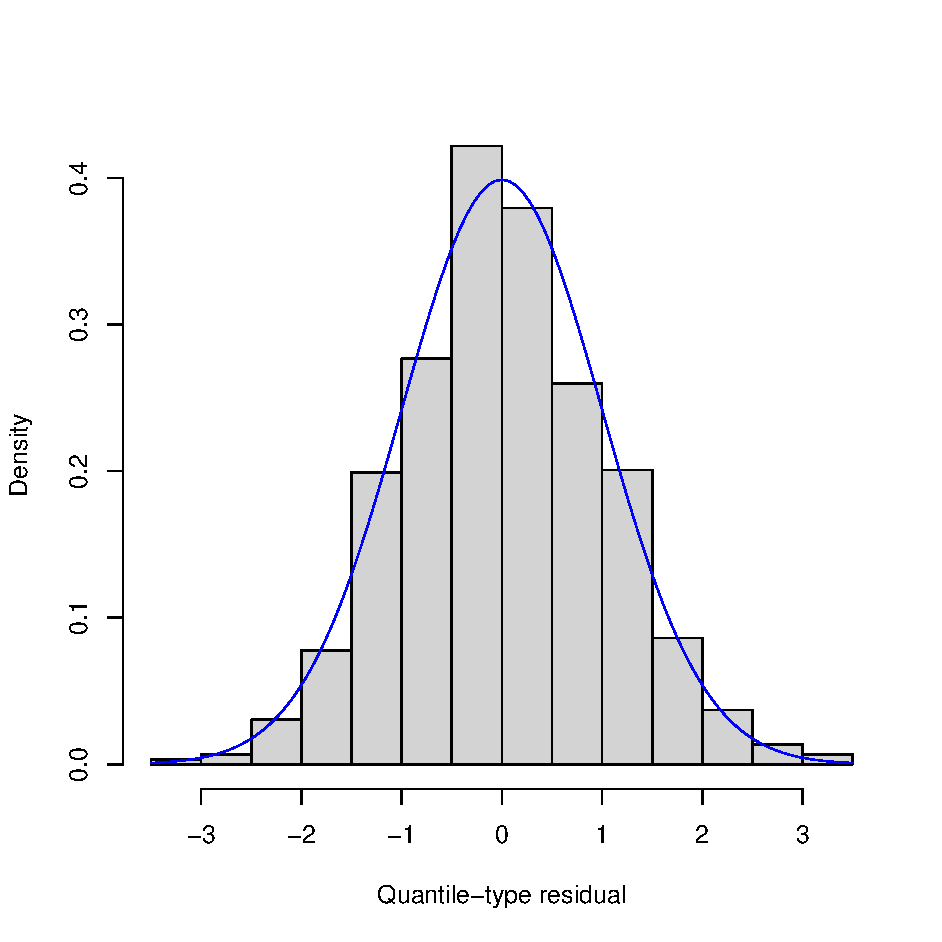
\includegraphics[width=6.5cm]{figures/hist.pdf}
\caption{Diagnostic plots of the quantile-type residuals for the ${\rm TAR}(3;\bm{p}=(5,5,5))$ model with Laplace innovations: Normal Q-Q plot (a) and histogram (b).}
\label{qq}
\end{figure}
The autocorrelation and partial autocorrelation functions of the quantile-type residuals can easily be obtained using \code{acf(res[["full"]])} and \code{pacf(res[["full"]])}, respectively. The selected TAR model, characterized by three regimes and Laplace innovations, extends the specification previously considered by \cite{CN17}. This result illustrates the advantages of the \CRANpkg{mtarm} framework, which enables the joint exploration of alternative regime structures and non-Gaussian innovation distributions. In this application, the additional modeling flexibility leads to a specification that achieves superior empirical performance while providing a richer characterization of the underlying hydrological dynamics.

\subsubsection{Convergence diagnostics}
Geweke's convergence diagnostic, implemented in the routine \code{geweke\_diag()} of the package \CRANpkg{coda}, was originally proposed by \cite{G92}. The following code uses the wrapper function \code{geweke\_diagTAR()} provided by \CRANpkg{mtarm} to apply \code{geweke\_diag()} to each MCMC chain obtained from the fitted ${\rm TAR}(3;\bm{p}=(5,5,5))$ Laplace model. This procedure yields the corresponding $z$-scores that form the basis of Geweke’s convergence assessment.
\begin{example}
> geweke_diagTAR(models[["Laplace.3.5"]])

Fraction in 1st window = 0.1
Fraction in 2nd window = 0.5

Thresholds:
Threshold.1 Threshold.2 
    -1.0652     -1.9642 

Regime 1

Autoregressive coefficients:
                  Bedon  LaPlata
(Intercept)    -1.08629 -0.14971
Bedon.lag(1)   -0.50880  0.70745
LaPlata.lag(1)  0.33666 -0.40158
Bedon.lag(5)    0.90577 -0.74717
LaPlata.lag(5) -0.46920  0.45755

Scale parameter:
           Bedon   LaPlata
Bedon   0.684164  0.059843
LaPlata 0.059843 -0.544754


Regime 2

Autoregressive coefficients:
                  Bedon  LaPlata
(Intercept)    -0.90517 -0.24451
Bedon.lag(1)    0.81444  2.10698
LaPlata.lag(1) -1.27630 -1.97840
Bedon.lag(5)    1.46737 -0.12233
LaPlata.lag(5)  1.17324  1.13680

Scale parameter:
           Bedon  LaPlata
Bedon    0.42967 -0.45240
LaPlata -0.45240  0.38793


Regime 3

Autoregressive coefficients:
                  Bedon  LaPlata
(Intercept)    -0.22473  1.48287
Bedon.lag(1)   -1.88483 -0.51478
LaPlata.lag(1)  1.97141 -0.93629

Scale parameter:
         Bedon LaPlata
Bedon   1.1593 1.51684
LaPlata 1.5168 0.80106
\end{example}
In most cases, the absolute values of the resulting $z$-scores are small relative to the $99.5\%$ quantile of the standard normal distribution. Consequently, at the $1\%$ significance level, Geweke's diagnostic provides not enough evidence against the convergence of the Markov chains. 
In addition, the \CRANpkg{mtarm} package provides the wrapper function \code{geweke\_plotTAR()}, which applies \code{geweke.plot()} from the \CRANpkg{coda} package to each MCMC chain generated for the fitted ${\rm TAR}(3;\bm{p}=(5,5,5))$ model with Laplace innovations, thereby providing a graphical assessment of convergence for all model parameters.

\begin{example}
> geweke_plotTAR(models[["Laplace.3.5"]])
\end{example}

To assess the mixing and sampling efficiency of the MCMC algorithm, the \code{effectiveSize\_TAR()} function computes the effective sample size (ESS) for all parameters estimated in an \code{mtar} object. The ESS measures the amount of independent information contained in the posterior sample after accounting for autocorrelation, making it a useful diagnostic for evaluating MCMC efficiency. The following code computes this diagnostic:

\begin{example}
> effectiveSize_TAR(models[["Laplace.3.5"]])

Thresholds:
Threshold.1 Threshold.2 
     8.8078     38.5229 

Regime 1
Autoregressive coefficients:
                 Bedon LaPlata
(Intercept)    1718.53  1126.2
Bedon.lag(1)   1043.34  1301.9
LaPlata.lag(1) 1352.69  1159.9
Bedon.lag(5)    908.21  1431.4
LaPlata.lag(5) 1240.61  1224.7

Scale parameter:
         Bedon LaPlata
Bedon   1785.1  2029.6
LaPlata 2029.6  1758.3

Regime 2
Autoregressive coefficients:
                 Bedon  LaPlata
(Intercept)    324.056  709.963
Bedon.lag(1)   240.927  138.885
LaPlata.lag(1) 506.795  144.089
Bedon.lag(5)    65.441 1309.136
LaPlata.lag(5) 365.276   42.178

Scale parameter:
         Bedon LaPlata
Bedon   1620.0  2059.3
LaPlata 2059.3  1752.9


Regime 3
Autoregressive coefficients:
                 Bedon LaPlata
(Intercept)    1101.19  1099.7
Bedon.lag(1)    634.62  1185.8
LaPlata.lag(1) 1022.89  1294.8

Scale parameter:
         Bedon LaPlata
Bedon   1719.5  1940.2
LaPlata 1940.2  1777.4
\end{example}

The output provides a useful summary of the sampling efficiency achieved by the MCMC algorithm. The scale parameters and most autoregressive coefficients—particularly those associated with Regimes 1 and 3—exhibit relatively large effective sample sizes, often exceeding 1000 draws, indicating good posterior exploration and satisfactory mixing. In contrast, the threshold parameters and a small number of coefficients in Regime 2 (e.g., \code{Bedon.lag(5)} and \code{LaPlata.lag(5)}) display comparatively lower ESS values. Such behavior is not unexpected in threshold autoregressive models, as threshold parameters are typically more challenging to estimate due to the regime-switching nature of the likelihood function \citep{VANEGAS2025}. Nevertheless, the ESS diagnostic provides valuable information for assessing the quality of the posterior sample and identifying parameters that may require additional simulation effort. In practice, if higher precision is desired for the slower-mixing components, the user may consider increasing the MCMC chain length or modifying the thinning strategy.

\subsubsection{Forecasting}
The following code generates forecasts of the river flows and their corresponding $90\%$ prediction intervals for the period from April 5, 2009, to April 14, 2009, conditional on the observed rainfall values over the same horizon. 

\begin{example}
> set.seed(0220)
> out <- predict(models[["Laplace.3.5"]], newdata=future.obs, n.ahead=nrow(future.obs), 
+                credible=0.9, row.names=Date)
> round(cbind(out[["summary"]][,c(1:3)], Bedon=future.obs[,"Bedon"]),2)

           Bedon.Mean Bedon.Lower Bedon.Upper Bedon
2009-04-05       9.79        7.08       12.30  9.46
2009-04-06      14.11        6.57       22.91 10.40
2009-04-07      17.04        7.77       27.12 13.24
2009-04-08      14.78        6.54       22.59 11.36
2009-04-09      13.33        5.95       20.63 11.17
2009-04-10      12.29        5.69       19.51 10.59
2009-04-11      15.75        6.72       25.47 11.46
2009-04-12      14.72        6.52       22.86 12.45
2009-04-13      12.73        6.17       19.30 11.46
2009-04-14      11.26        5.52       16.44 11.07
>
> round(cbind(out[["summary"]][,c(4:6)], LaPlata=future.obs[,"LaPlata"]),2)

           LaPlata.Mean LaPlata.Lower LaPlata.Upper LaPlata
2009-04-05        24.15         16.80         31.22   19.60
2009-04-06        34.33          4.94         64.76   25.26
2009-04-07        38.69          3.82         74.13   42.28
2009-04-08        32.97          8.36         55.74   33.45
2009-04-09        29.68         10.32         48.07   32.40
2009-04-10        27.51         10.66         43.71   25.17
2009-04-11        35.73          1.42         67.58   42.73
2009-04-12        31.80          8.48         55.34   29.27
2009-04-13        27.20          9.02         44.12   27.38
2009-04-14        24.20         10.99         38.26   25.82
\end{example}
The river flow forecasts closely track the observed values, and all true observations lie within the associated $90\%$ prediction intervals. Figure \ref{fore} displays the last 300 observations of the Bedon and La Plata river flows, shown as solid black lines. Ten-step-ahead forecasts are indicated by dashed black lines, while the corresponding $90\%$ prediction intervals are represented by light gray shaded bands. The following code produces this figure.
\begin{example}
> plot(out,last=300,
+          historical=list(type="l",col="black",lty=1),
+          forecasts=list(type="l",col="black",lty=3,ylab=rep("Cubic meters per second",2)),
+          forecasts.PI=list(col="light gray",border=NULL))
\end{example}

\begin{figure}[!h]
\centering
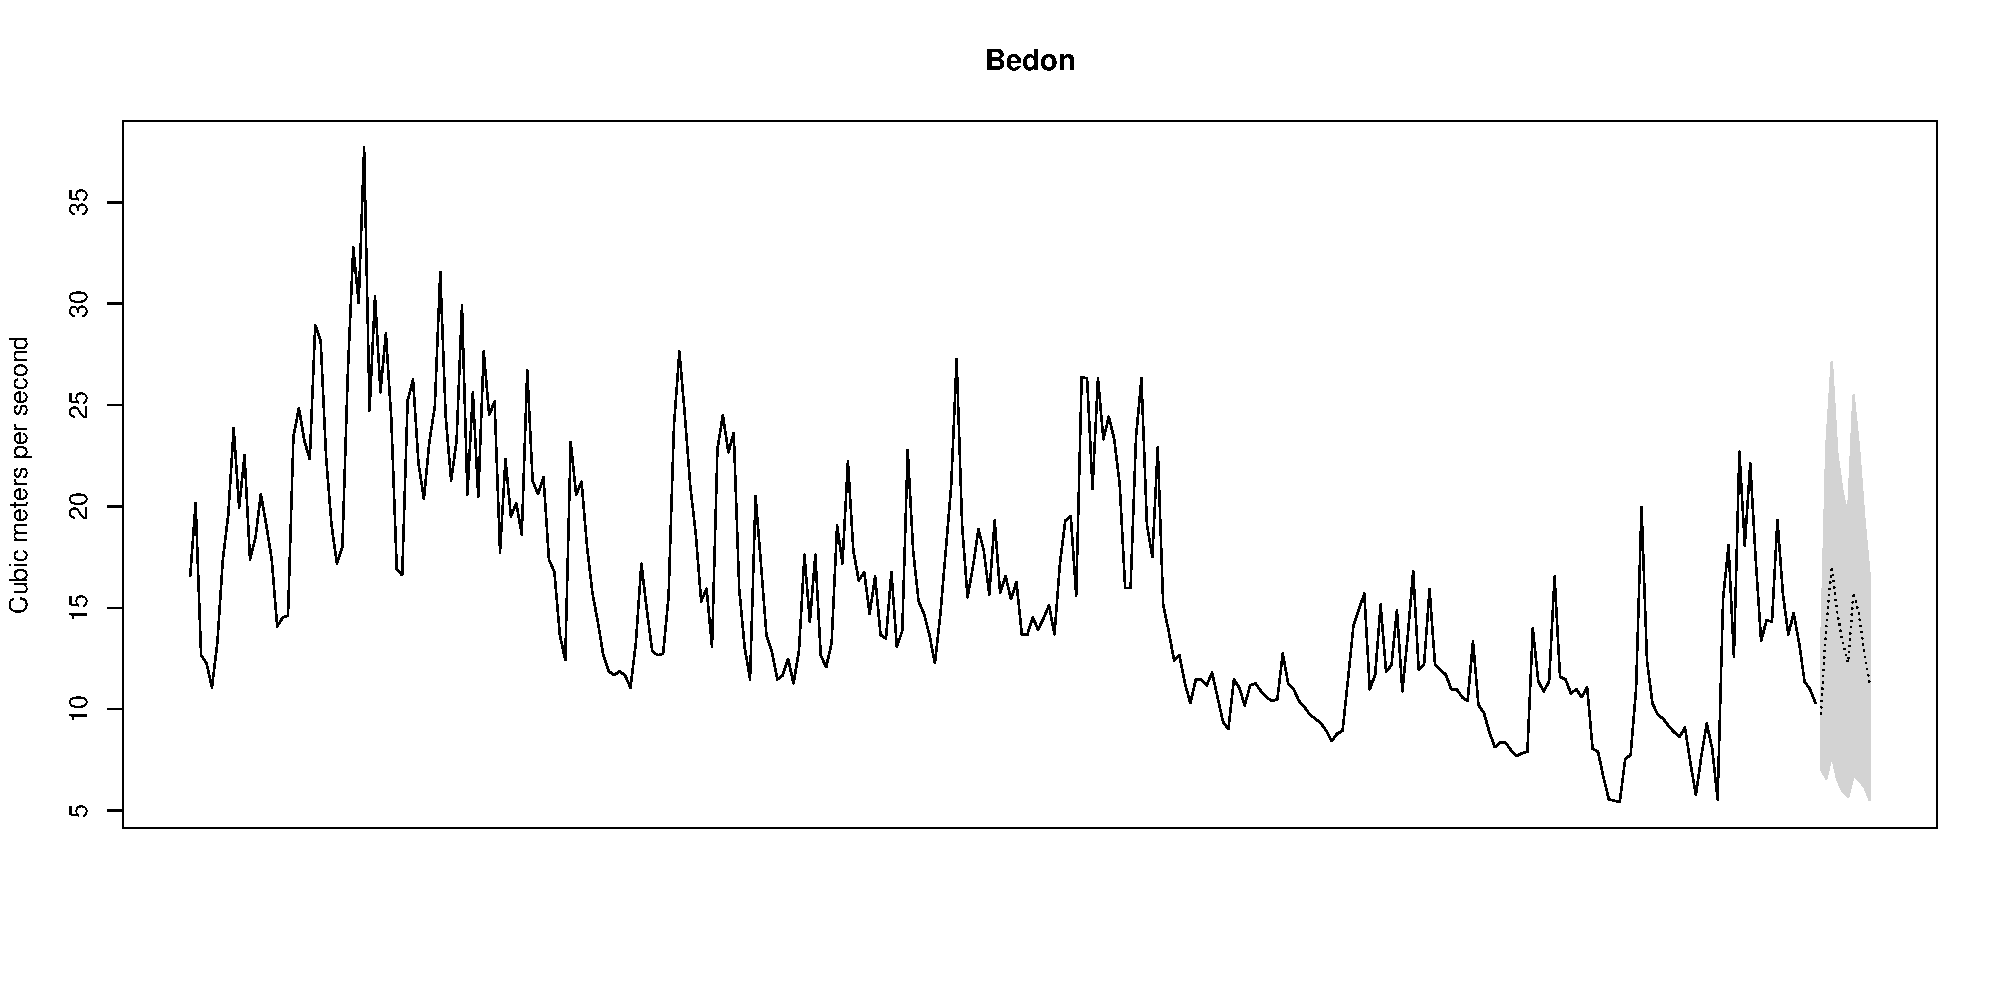
\includegraphics[width=12cm]{figures/Bedon}\\
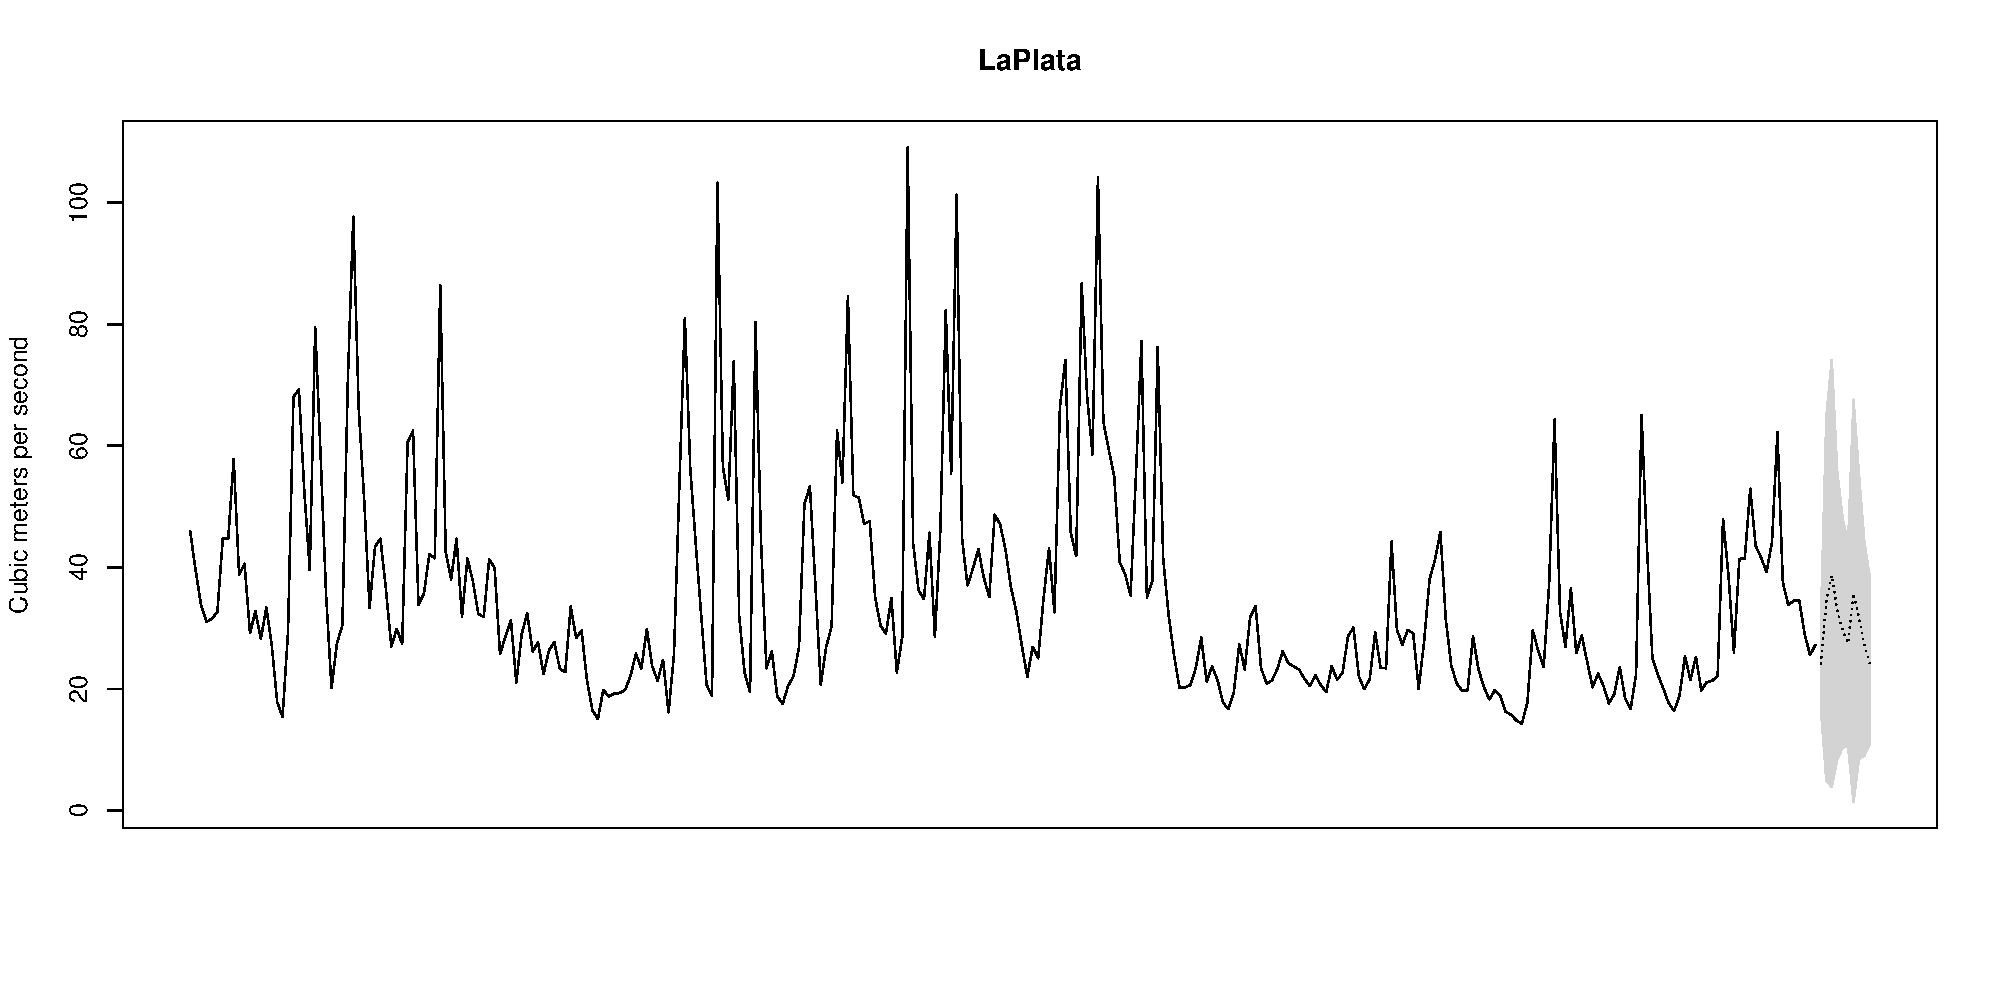
\includegraphics[width=12cm]{figures/LaPlata}
\caption{Observed and forecasted Bedon River flow (a) and La Plata River flow (b). The last 300 observations are shown together with 10-step-ahead forecasts and their associated $90\%$ prediction intervals.}
\label{fore}
\end{figure}
The \code{predict()} method for \code{mtar} objects generates point forecasts and predictive intervals for the multivariate response series. These forecasts are obtained from the posterior predictive distribution, thereby incorporating parameter uncertainty into the prediction process.
Those forecasts are obtained from known or previously forecasted values for the input time series (if there is one in the fitted model) and the exogenous time series (if there is one in the fitted model) for the time points at which forecasts of the output time series are requested. This method can also be used to evaluate the out-of-sample predictive performance of a fitted model. For this purpose, it computes several forecast accuracy measures, including the Absolute Error (AE), Absolute Percentage Error (APE), and Squared Error (SE), which assess point forecast accuracy, as well as the log-score and Energy Score, which evaluate the quality of the predictive distribution. The main arguments of the \code{predict()} method are as follows:

\begin{itemize}
\item \underline{\bf object}. An \code{mtar}-type object resulting from a call to the routine \code{mtar()}, that is, an object in which the results of a fitted TAR model are stored.
\item \underline{\bf newdata}. A \code{data.frame}-type object with rows representing time points, arranged in ascending order with respect to time, which includes the future values for the threshold time series (if there is one in the fitted model) and the exogenous time series (if there is one in the fitted model). The columns composing those series must be named equal to those used to call the routine \code{mtar()}.

\item \underline{\bf n.ahead}. It is an integer value specifying the number of desired forecast steps.

\item \underline{\bf row.names}. It is an optional column in \code{newdata} with the labels for the time points for which the forecast is requested.

\item \underline{\bf credible}. The credible level for the prediction intervals. By default, \code{credible} is set to $0.95$.

\item \underline{\bf out.of.sample}. It is a logical type argument. If \code{TRUE} then the AE, APE, SE, log-score and Energy Score values are computed for each requested forecast step. Therefore, the \code{data.frame}-type object specified in the argument \code{newdata} must include the actual values of the output time series stored in columns whose names are equal to those used to call the routine \code{mtar()}.

\item \underline{\bf rolling}. A positive integer specifying the size of the rolling window used for out-of-sample forecasting with fixed model parameters when \code{out.of.sample = TRUE}. By default, \code{rolling = NULL}, indicating that forecasts are generated without updating the estimation window.
\end{itemize}

The method \code{predict()} returns a list-type object that includes the following objects: $(i)$ \code{summary}, a matrix with the forecasts and their associated prediction intervals; and $(ii)$ the objects \code{LS}, \code{ES}, \code{AE}, \code{APE}, \code{SE}, \code{Width} and \code{CR} provided that \code{out.of.sample=TRUE}. 

\subsubsection{Simulating from a TAR model}

To illustrate the full flexibility of the simulation framework, we next describe the complete syntax of the \code{simtar()} function and present several alternative simulation settings.
\begin{example}
> args(simtar)
function(n, k=2, ars=ars(), Intercept=TRUE, trend=c("none","linear","quadratic"), 
         nseason=NULL, parms, delay=0, thresholds=NULL, t.series=NULL, 
         ex.series=NULL, dist=c("Gaussian","Student-t","Hyperbolic","Laplace",
         "Slash","Contaminated normal","Skew-Student-t","Skew-normal"), 
         skewness=NULL, extra=NULL, setar=NULL, Verbose=TRUE)
\end{example}    
The function \code{simtar()} simulates multivariate time series whose behavior follows a pre-specified TAR model. As shown in Table~\ref{simtar}, the routine is sufficiently flexible to also accommodate special cases such as SETAR and VAR models. In addition, it includes an optional logical argument that controls whether a summary description of the simulated TAR model is printed.

\begin{table}[!ht]
{\small
\begin{center}
\begin{tabular}{llll} 
 \hline
   &  Argument &  Type & Description\\ \hline
$T$      & \code{n} & Integer & Length of the time series\\
$k$      &  \code{k} & Integer & Dimension of the output series\\
$l$ & \multirow{4}{*}{\code{ars}} & \multirow{4}{*}{List} & \multirow{4}{*}{Same as the argument \code{ars} of \code{mtar()}}\\
$\bm{p}\!=\!(p_1,\ldots,p_l)$ &                       &                                          &  \\
$\bm{q}\!=\!(q_1,\ldots,q_l)$ &                       &                                          &  \\
$\bm{d}\!=\!(d_1,\ldots,d_l)$ &                       &                                          &  \\
$h$ & \code{delay} & Non-negative integer & Delay parameter\\
$\bm{c}\!=\!(\!c_1,\ldots,c_{l-1}\!)$ & \code{thresholds}& Vector of size $l-1$ & Threshold values for the input series \\
                  & \code{setar} & Integer in $\{1,\ldots,k\}$ & Same as the argument \code{setar} of \code{mtar()}\\
$z_t$ & \code{t.series}& Matrix of size $T^*\!\times 1\,\dagger$ & Threshold series \\
$\bm{x}_t$ & \code{ex.series}& Matrix of size $T^*\!\times r\,\dagger$ & Exogenous series\\
$\bm{\epsilon}_t \myeq $ & \code{dist}& Character & Same as the argument \code{dist} of \code{mtar()}\\
$\bm{\lambda}=(\lambda_1,\ldots,\lambda_k)^{\!\top}$ & \code{skewness} & Vector of size $k$ & Skewness parameter\\ 
$\nu$  & \code{extra} & Numeric  & Extra parameter value\\
\multirow{3}{*}{$\bm{\phi}_0^{^{(j)}}\!,\,j=1,\ldots,l$} & \code{Intercept} & Logical & Same as the argument \code{Intercept} of \code{mtar()}\\
 & \code{trend} & Character & Same as the argument \code{trend} of \code{mtar()}\\
 & \code{nseason} & Integer & Same as the argument \code{nseason} of \code{mtar()}\\
$\bm{\phi}_0^{^{(j)}}\!,\bm{\phi}_1^{^{(j)}}\!,\ldots,\bm{\phi}_{p_j}^{^{(j)}},$ & \multirow{4}{*}{\code{parms}} & \multirow{4}{*}{List composed of $l$ lists$\,\ddagger$} & \multirow{4}{*}{Location and scale parameter values}\\
$\bm{\beta}_1^{^{(j)}}\!,\ldots,\bm{\beta}_{q_j}^{^{(j)}},\bm{\delta}_1^{^{(j)}}\!,$ &    &    & \\
$\ldots,\bm{\delta}_{d_j}^{^{(j)}}$ and $\bm{\Sigma}_j$  &    &    & \\
 for $j=1,\ldots,l$  &    &    & \\
\hline
\end{tabular}
\end{center}
\vspace{-3mm}
{\footnotesize $\dagger$\, $T^*=T+{\rm max}\{p_1,\ldots,p_{l},q_1,\ldots,q_{l},d_1,\ldots,d_{l},h\}$\\
$\ddagger$\, The $j$-th list, named \code{j}, is composed of 2 matrices. The first one, named \code{location}, stores the location parameters, that is,
$(\bm{\phi}_0^{^{(j)}},\bm{\phi}_1^{^{(j)}},\ldots,\bm{\phi}_{p_j}^{^{(j)}},\bm{\beta}_1^{^{(j)}},\ldots,\bm{\beta}_{q_j}^{^{(j)}},
\bm{\delta}_1^{^{(j)}},\ldots,\bm{\delta}_{d_j}^{^{(j)}})^{\!\top}$. The second matrix, named \code{scale}, stores the scale parameters, that is,
$\bm{\Sigma}_j$.}
\caption{Arguments of the \code{simtar()} function.}
\label{simtar}}
\end{table}

For example, the following code simulates a bivariate time series of size 2000 whose behavior follows a ${\rm VAR}(2)$ model with a linear time trend, four seasonal periods and a multivariate Laplace distribution describing the noise process. In addition, the elements of the matrix of location parameters (i.e., $(\bm{\phi}_0,\bm{\phi}_1,\bm{\phi}_2)^{\!\top}$) are randomly generated from $(1-2W)\times V$, where $W\sim {\rm Bernoulli}(0.5)$ and $V\sim{\rm Beta}(4,16)$ are independent random variables, whereas the scale parameter (i.e., $\bm{\Sigma}$) is set as a diagonal matrix with elements randomly generated from the ${\rm Exponential}(1)$.

\begin{example}
> set.seed(0220)
> n <- 2000
> k <- 2
> myars <- ars(nregim=1, p=2)
> Intercept <- TRUE
> trend <- "linear"
> nseason <- 4
> dist <- "Laplace"
> deterministic <- Intercept + switch(trend,"linear"=1,"quadratic"=2,"none"=0) + 
+                              ifelse(is.null(nseason),0,nseason-1)
> parms <- list()
> parms[[1]] <- list()
> np <- deterministic + myars$p*k
> parms[[1]]$location <- ifelse(runif(np*k)<=0.5,1,-1)*rbeta(np*k,shape1=4,shape2=16)
> parms[[1]]$location <- matrix(parms[[1]]$location,np,k)
> parms[[1]]$scale    <- rexp(k,rate=1)*diag(k)
>
> myVAR <- simtar(n=n, k=k, ars=myars, dist=dist, Intercept=Intercept, trend=trend, 
+                 nseason=nseason, parms=parms, Verbose=TRUE)

Sample size          : 2000  time points
Output Series        : Y1 | Y2
Error Distribution   : Laplace
Number of regimes    : 1
Deterministics       : Intercept + a linear time trend + 4 seasonal periods
Autoregressive orders: 2 in each regime

Regime  1 :

Autoregressive coefficients
     Intercept     linear   season.2  season.3   season.4        phi_1                   phi_2
Y1  0.10794066 -0.2298236 -0.2158606 0.2096798  0.1300396 | -0.4496798 -0.1437272 | 0.23212132
Y2 -0.06531457  0.1238318 -0.3082912 0.2128472 -0.3215392 | -0.2693481  0.1936919 | 0.06750432

Y1 0.06180898 |
Y2 0.20084720 |

Scale parameter
         Y1        Y2
Y1 2.856245 0.0000000
Y2 0.000000 0.6909536

> str(myVAR)
'data.frame':   2002 obs. of  3 variables:
 $ Y1    : num  -0.652 1.943 -14.48 5.515 -12.308 ...
 $ Y2    : num  0.694 -0.424 -4.698 4.514 -4.043 ...
 $ Regime: num  NA NA 1 1 1 1 1 1 1 1 ...
 \end{example}    
The model can be fitted to the simulated time series using the following instructions.
\begin{example}
> fit <- mtar( ~ Y1 + Y2, data=myVAR, ars=myars, Intercept=Intercept, trend=trend, 
+                nseason=nseason, dist=dist, n.burnin=2000, n.sim=3000, n.thin=2)
\end{example}
Similarly, the following code simulates a bivariate series $\{\bm{Y}_t\}_{_{t\geq 1}}$, where $\bm{Y}_t=(Y_{1,t},Y_{2,t})^{\!\top}$, according to a SETAR model with the following characteristics: $(i)$ there are 2 regimes; $(ii)$ the location parameter of the conditional distribution of $\bm{Y}_t$ is $\bm{\phi}_0^{^{(1)}} + \bm{\phi}_1^{^{(1)}}y_{t-1}$ in Regime 1, and $\bm{\phi}_0^{^{(2)}} + \bm{\phi}_1^{^{(2)}}y_{t-1} + \bm{\phi}_2^{^{(2)}}y_{t-2}$ in Regime 2; $(iii)$ the threshold time series corresponds to the second component of $\bm{Y}_t$, that is, $Y_{2,t}$; $(iv)$ the threshold value is 0.3 and the delay parameter $h$ is $1$, so that $\bm{Y}_t$ is in Regime 1 if $Y_{2,t-1}\leq 0.3$, and it is in Regime 2 if $Y_{2,t-1} > 0.3$; $(v)$ the noise process distribution is Student-$t$ with $4$ degrees of freedom, that is, $\bm{\epsilon}_t \myeq \text{Student-}t({\bf 0},\bm{I},4)$, so that its mean and variance-covariance matrix are finite, which implies that both the conditional mean and the conditional variance-covariance matrix of $\bm{Y}_t$ are also finite; and $(vi)$ the length of the series is $2000$. The values of the location parameters of the first (i.e., $(\bm{\phi}_0^{^{(1)}},\bm{\phi}_1^{^{(1)}})^{\!\top}$) and second (i.e., $(\bm{\phi}_0^{^{(2)}},\bm{\phi}_1^{^{(2)}},\bm{\phi}_2^{^{(2)}})^{\!\top}$) regimes are stored in matrices named \code{parms[[1]]\$location} and \code{parms[[2]]\$location}, respectively. Similarly, the values of the scale parameters of the first (i.e., $\bm{\Sigma}_1$) and second (i.e., $\bm{\Sigma}_2$) regimes are stored in matrices named \code{parms[[1]]\$scale} and \code{parms[[2]]\$scale}, respectively.

\begin{example}
> set.seed(0220)
> n <- 2000
> k <- 2
> myars <- ars(nregim=2, p=c(1,2))
> setar <- 2
> thresholds <- 0.3
> delay <- 1
> Intercept <- TRUE
> dist <- "Student-t"
> extra <- 4
> parms <- list()
> for(j in 1:myars$nregim){
+     np <- Intercept + myars$p[j]*k
+     parms[[j]] <- list()
+     parms[[j]]$location <- ifelse(runif(np*k)<=0.5,1,-1)*rbeta(np*k,shape1=4,shape2=16)
+     parms[[j]]$location <- matrix(parms[[j]]$location,np,k)
+     parms[[j]]$scale    <- rexp(k,rate=1)*diag(k)
> }
> mySETAR <- simtar(n=n, k=k, ars=myars, Intercept=Intercept, setar=setar, parms=parms, 
+              thresholds=thresholds, delay=delay, dist=dist, extra=extra, Verbose=TRUE)

Sample size          : 2000  time points
Output Series        : Y1 | Y2
Threshold Series     : Y2 with a delay equal to 1
Error Distribution   : Student-t(4)
Number of regimes    : 2
Deterministics       : Intercept
Autoregressive orders: 1, 2

Thresholds                   
Regime 1 (-Inf,0.3]
Regime 2  (0.3,Inf)

Regime  1 :
Autoregressive coefficients
   Intercept        phi_1             
Y1 0.3391083 | -0.1423164 -0.1146139 |
Y2 0.2180902 |  0.1641546 -0.1079407 |

Scale parameter
         Y1        Y2
Y1 3.774202 0.0000000
Y2 0.000000 0.3872779

Regime  2 :
Autoregressive coefficients
    Intercept        phi_1                  phi_2             
Y1 -0.1898829 | -0.2227718  0.2326686 | 0.1879023 0.09084321 |
Y2 -0.1567592 |  0.3272486 -0.1928849 | 0.2885574 0.29326418 |

Scale parameter
          Y1        Y2
Y1 0.6175893 0.0000000
Y2 0.0000000 0.7249159

> str(mySETAR)
'data.frame':   2002 obs. of  3 variables:
 $ Y1    : num  0.505 0.307 1.911 -1.652 0.468 ...
 $ Y2    : num  -2.357 0.188 0.452 -1.218 -1.021 ...
 $ Regime: num  NA NA 1 2 1 1 1 1 1 1 ...
\end{example}

The simulated time series is stored in a \code{data-frame} named \code{mySETAR}. The ${\rm SETAR}(\bm{p}=(1,2))$ Student-$t$ model can be fitted to the simulated time series using the following instructions.
\begin{example}
> fit <- mtar( ~ Y1 + Y2, data=mySETAR, ars=myars, setar=setar, dist=dist, 
+              n.burnin=2000, n.sim=3000, n.thin=2)
\end{example}

\section{River flows in Iceland}
The data consist of two daily river flow series from Iceland, originally reported by \cite{T90}, and are available in the \code{iceland.rf} dataset included in \CRANpkg{mtarm}. The corresponding variables are summarized in Table~\ref{td2}. While \cite{T90} described the geographical and meteorological characteristics of the rivers and analyzed each series separately, \cite{T98} later adopted a multivariate perspective by jointly modeling both river flow series. The response vector $\bm{Y}_t=(Y_{1,t},Y_{2,t})^{\!\top}$ consists of the daily flows of the Jökulsá Eystri $(Y_{1,t})$ and Vatnsdalsá $(Y_{2,t})$ rivers, measured in cubic meters per second $(m^3/s)$, over the period from January 1, 1972, to December 31, 1974, yielding a total of 1096 observations. The explanatory variables include daily precipitation $(X_t)$, measured in millimeters $(mm)$, and daily temperature $(Z_t)$, measured in degrees Celsius $(^{\circ}\mathrm{C})$, both recorded at the Hveravellir meteorological station. Precipitation values correspond to the total rainfall accumulated during the preceding 24 hours and recorded at 9:00 A.M. Given the subarctic climate of the region, river flow dynamics are expected to be strongly influenced by temperature-dependent processes such as snow accumulation and snowmelt. Consequently, temperature $(Z_t)$ is a natural choice for the threshold variable in a multivariate TAR model, allowing the relationship between river flows and meteorological conditions to vary across distinct thermal regimes. To assess the benefits of incorporating such nonlinearities, standard VAR models are also considered as linear benchmark specifications. Model comparison is based on both in-sample fit criteria and out-of-sample predictive performance, thereby providing a comprehensive evaluation of the competing models.

\begin{table}[!ht]
{\small
\begin{center}
\begin{tabular}{lll} 
 \hline
Column &  Role &  Description\\ \hline
\code{Date}           & Labels for time points                & Dates when measurements were taken\\ 
\code{Jokulsa}        & First component of the output series  & Jökulsá Eystri river flow, in $m^3\!/\!s$\\
\code{Vatnsdalsa}     & Second component of the output series & Vatnsdalsá river flow, in $m^3\!/\!s$\\
\code{Precipitation}  & Exogenous series                      & Rainfall, in $mm$\\
\code{Temperature}    & Threshold series                      & Temperature, in degrees Celsius ($^{\circ}\text{C}$)\\ 
 \hline
\end{tabular}
\end{center}
\caption{Description of the variables in the \code{iceland.rf} dataset included in the \CRANpkg{mtarm} package.}
\label{td2}}
\end{table}
Similar to \cite{T98}, the observed series are analyzed here using a TAR$(2;p=(15,15),q=(4,4),d=(2,2))$ model, that is,
$$\bm{Y}_t=\sum\limits_{j=1}^2 I(Z_{t-h}\in(c_{j-1},c_j])\Big(\!\bm{\phi}_0^{^{(j)}}+\sum\limits_{i=1}^{15}\bm{\phi}_i^{^{(j)}}\bm{Y}_{t-i}+\sum\limits_{i=1}^{4}\bm{\beta}_i^{^{(j)}}\!X_{t-i}+\sum\limits_{i=1}^{2}\bm{\delta}_i^{^{(j)}}\!Z_{t-i}+\bm{\epsilon}_{t_j}\!\Big).$$

\subsection{Model estimation}
The following code fits a TAR$(2; \bm{p}=(15,15), \bm{q}=(4,4), \bm{d}=(2,2))$ model to the output series under four alternative assumptions for the noise process distribution: Gaussian, Student-$t$, skew-normal, and skew-$t$. In each specification, the relevant lags of the output series $\{\bm{Y}_t\}_{t\geq 1}$, the exogenous series $\{X_t\}_{t\geq 1}$, and the threshold series $\{Z_t\}_{t\geq 1}$ are selected using the Stochastic Search Variable Selection (SSVS) procedure. Furthermore, the last 10 observations of the sample period (from December 22, 1974, to December 31, 1974) are excluded from the estimation stage, as they are subsequently used to evaluate out-of-sample predictive performance.
\begin{example}
> data(iceland.rf)
> str(iceland.rf)
'data.frame':   1096 obs. of  5 variables:
 $ Vatnsdalsa   : num  16.1 19.2 14.5 11 13.6 12.5 10.5 10.1 9.68 9.02 ...
 $ Jokulsa      : num  30.2 29 28.4 27.8 27.8 27.8 27.8 27.8 27.8 27.3 ...
 $ Precipitation: num  8.1 4.4 7 0 0 0 1.9 1.2 0 0.1 ...
 $ Temperature  : num  0.9 1.6 0.1 0.6 2 0.8 1.4 1.3 2.2 0.1 ...
 $ Date         : Date, format: "1972-01-01" "1972-01-02" "1972-01-03" ...
>
> set.seed(0220)
> models <- mtar_grid(~ Jokulsa + Vatnsdalsa | Temperature | Precipitation, data=iceland.rf, 
+                     subset={Date<="1974-12-21"}, row.names=Date, dist=c("Gaussian",
+                     "Student-t","Skew-normal","Skew-Student-t"), nregim.min=2, nregim.max=2,
+                     p.min=15, p.max=15, q.min=4, q.max=4, d.min=2, d.max=2, n.burnin=5000, 
+                     n.sim=4000, n.thin=2, ssvs=TRUE, plan_strategy="multisession")
>
> models

Sample size          : 1071 time points (1972-01-16 to 1974-12-21)
Output Series        : Jokulsa    |    Vatnsdalsa
Threshold Series (TS): Temperature
Exogenous Series (ES): Precipitation
Error Distribution   : Gaussian, Skew-normal, Skew-Student-t, Student-t
Number of regimes    : 2
Deterministics       : Intercept  
Autoregressive order : 15
Maximum lag for ES   : 4
Maximum lag for TS   : 2
\end{example}

\subsection{Model selection}
For each fitted model, both in-sample and out-of-sample predictive performance measures are computed. The in-sample measures include the DIC and WAIC, whereas the out-of-sample measures consist of the average log-score, the average Energy Score, the empirical coverage rate, and the average width of the $95\%$ prediction intervals.
\begin{example}
> DICs <- DIC(models)
> WAICs <- WAIC(models)
>
> round(cbind(DICs,WAICs),2)
                             DIC     WAIC
Gaussian.2.15.4.2       10263.25 10489.02
Skew-normal.2.15.4.2     9530.98  9747.58
Skew-Student-t.2.15.4.2  7660.34  7687.53
Student-t.2.15.4.2       7627.35  7724.44

> future.obs <- subset(iceland.rf, Date>"1974-12-21") 
> set.seed(0220)
> oos <- out_of_sample(models, credible=0.95, newdata=future.obs, 
+                      n.ahead=nrow(future.obs), FUN=mean)
>
> round(oos[,c(1,2,9:12)], 2)           
                    Log.Score Energy.Score Jokulsa.Width Vatnsdalsa.Width Jokulsa.CR Vatnsdalsa.CR
Gaussian.2.15.4.2        3.02         1.69          9.63             6.08          1             1
Skew-normal.2.15.4.2     2.56         1.15          6.46             3.91          1             1
Skew-Student-t.2.15.4.2  3.96         1.95         11.28             9.09          1             1
Student-t.2.15.4.2       2.61         1.70         10.33             8.29          1             1
\end{example}
The competing models exhibit some variation in their rankings across the evaluation criteria. According to the DIC and WAIC, the specification with skew-Student-$t$/Student-$t$ innovations provides the best overall fit, with the Student-$t$/skew-Student-$t$ model performing nearly as well. In contrast, both the average log-score and the average Energy Score favor the specification with skew-normal innovations, while the Student-$t$ model consistently ranks second. The comparison based on the $95\%$ prediction intervals is less informative because all models achieve complete empirical coverage. Nevertheless, the skew-normal specification produces substantially narrower prediction intervals on average, indicating greater predictive sharpness without compromising calibration. Overall, the results reveal a trade-off between in-sample fit and out-of-sample predictive performance. Although the skew-Student-$t$ and Student-$t$ specifications are preferred according to the information criteria, the skew-normal specification yields superior predictive accuracy together with more precise prediction intervals. Given the emphasis on forecasting performance, the skew-normal specification is selected for the subsequent analysis.

\subsection{Overview of the chosen model}
The preferred model is summarized below.
\begin{example}
> summary(models[["Skew-normal.2.15.4.2"]])

Sample size          : 1071 time points (1972-01-16 to 1974-12-21)
Output Series (OS)   : Jokulsa    |    Vatnsdalsa
Threshold Series (TS): Temperature with a estimated delay equal to 0
Exogenous Series (ES): Precipitation
Error Distribution   : Skew-normal
Number of regimes    : 2
Deterministics       : Intercept  
Autoregressive orders: 15 in each regime
Maximum lags for ES  : 4 in each regime
Maximum lags for TS  : 2 in each regime

Thresholds (Mean, HDI.Lower, HDI.Upper)
Regime 1 (-Inf,-0.45131] (-Inf,-0.4994] (-Inf,-0.40566]
Regime 2  (-0.45131,Inf)  (-0.4994,Inf)  (-0.40566,Inf)


Regime1:
     OS.lag(1)  OS.lag(2)  OS.lag(3)  OS.lag(4)  OS.lag(5)  OS.lag(6)  OS.lag(7) OS.lag(8) 
SSVS        1          1          1          0          0          0          0         0 
     OS.lag(9) OS.lag(10) OS.lag(11) OS.lag(12) OS.lag(13) OS.lag(14) OS.lag(15) ES.lag(1)
            0          0          1          0          0          0          0         0 
     ES.lag(2)  ES.lag(3)  ES.lag(4)  TS.lag(1)  TS.lag(2)
         0.02          0          0          0          0

Autoregressive coefficients
                      Mean  2(1-PD) HDI.Lower HDI.Upper    Mean  2(1-PD) HDI.Lower HDI.Upper
(Intercept)         7.82970 0.00001  7.05110  8.60872 |  2.16764 0.00001  1.85504  2.53065
Jokulsa.lag( 1)     0.51454 0.00001  0.43375  0.59311 | -0.05485 0.00001 -0.08455 -0.02651
Vatnsdalsa.lag( 1)  0.41706 0.00001  0.29846  0.53476 |  0.87652 0.00001  0.81374  0.93883
Jokulsa.lag( 2)     0.00961 0.82000 -0.06125  0.08595 |  0.02573 0.13150 -0.00644  0.06288
Vatnsdalsa.lag( 2) -0.20241 0.00200 -0.33230 -0.06691 | -0.20115 0.00001 -0.26561 -0.13553
Jokulsa.lag( 3)     0.12441 0.00001  0.07372  0.17434 |  0.00598 0.63100 -0.01854  0.03100
Vatnsdalsa.lag( 3) -0.08044 0.07800 -0.17010  0.01040 |  0.09105 0.00100  0.04060  0.14201
Jokulsa.lag(11)     0.05987 0.00001  0.03537  0.08581 |  0.00537 0.42750 -0.00744  0.01843
Vatnsdalsa.lag(11) -0.04732 0.01400 -0.08295 -0.01176 |  0.05106 0.00001  0.02942  0.06887

Scale parameter (Mean, HDI.Lower, HDI.Upper)
           Jokulsa Vatnsdalsa      Jokulsa Vatnsdalsa      Jokulsa Vatnsdalsa
Jokulsa    1.29030    0.15385    . 0.98590    0.07924    . 1.57325    0.23292
Vatnsdalsa 0.15385    0.20602    . 0.07924    0.14868    . 0.23292    0.26663

Regime2:
     OS.lag(1)  OS.lag(2)  OS.lag(3)  OS.lag(4)  OS.lag(5)  OS.lag(6)  OS.lag(7) OS.lag(8) 
SSVS        1          1        0.3        0.7          0          0          0         0  
     OS.lag(9) OS.lag(10) OS.lag(11) OS.lag(12) OS.lag(13) OS.lag(14) OS.lag(15) ES.lag(1) 
            0          0          0          0          0          0          0      0.01  
     ES.lag(2)  ES.lag(3)  ES.lag(4)  TS.lag(1)  TS.lag(2)
            0          0          0          1          1

Autoregressive coefficients
                      Mean  2(1-PD) HDI.Lower HDI.Upper    Mean  2(1-PD) HDI.Lower HDI.Upper
(Intercept)         3.61496 0.00001  1.74559  5.40196 |  2.43909 0.00001  1.84246  3.04396
Jokulsa.lag( 1)     1.04322 0.00001  0.95892  1.13108 |  0.00106 0.94150 -0.02486  0.02917
Vatnsdalsa.lag( 1)  0.79057 0.00001  0.50879  1.05482 |  1.21472 0.00001  1.11489  1.32856
Jokulsa.lag( 2)    -0.22844 0.00001 -0.38460 -0.10183 | -0.01011 0.53900 -0.04316  0.02164
Vatnsdalsa.lag( 2) -0.99689 0.00001 -1.42281 -0.58657 | -0.53671 0.00001 -0.76564 -0.37173
Jokulsa.lag( 4)    -0.02972 0.22750 -0.06799  0.02291 | -0.02065 0.02300 -0.03485 -0.00411
Vatnsdalsa.lag( 4)  0.52088 0.00001  0.36035  0.72024 |  0.26715 0.00001  0.20760  0.32753
Temperature.lag(1)  1.71978 0.00001  1.34312  2.08671 |  0.11227 0.07350 -0.00177  0.24110
Temperature.lag(2) -0.87721 0.00001 -1.22428 -0.57624 | -0.12042 0.02200 -0.22141 -0.01141

Scale parameter (Mean, HDI.Lower, HDI.Upper)
           Jokulsa Vatnsdalsa       Jokulsa Vatnsdalsa       Jokulsa Vatnsdalsa
Jokulsa    60.1243    5.01920    . 53.21215    3.37068    . 66.85740    6.81176
Vatnsdalsa  5.0192    6.34542    .  3.37068    5.62933    .  6.81176    7.14503

Skewness parameter
                        Mean    2(1-PD)  HDI.Lower HDI.Upper
lambda1              -1.13231   0.00150  -1.48391  -0.75087
lambda2              -0.86829   0.00001  -0.99011  -0.73948
\end{example}
The posterior mean estimates of the delay and threshold parameters for the selected model are $0$ and $-0.45$, respectively. These estimates suggest that the dynamics of the daily river flows depend on contemporaneous temperature values and on whether the temperature lies below or above the threshold of $-0.45 \,^{\circ}\text{C}$. Accordingly, Regime 1 corresponds to days with temperatures not exceeding $-0.45\,^{\circ}\text{C}$, whereas Regime 2 corresponds to days with temperatures above this level. The observations are distributed almost evenly across the two regimes, with 470 observations assigned to Regime 1 and 601 to Regime 2. Examination of the posterior means of the variable-selection indicators $\bm{\zeta}_1$ and $\bm{\zeta}_2$ reveals notable differences in the dynamic structure across regimes. In Regime 1, only the first, second and eleventh lags of $\{\bm{Y}_t\}_{t\geq 1}$ are selected, indicating that the current river flows are primarily explained by their recent past values. In contrast, Regime 2 exhibits a richer dependence structure: in addition to the first, second and fourth lags of $\{\bm{Y}_t\}_{t\geq 1}$, the first and second lags of the temperature series $\{Z_t\}_{t\geq 1}$ are also selected. Furthermore, the posterior means and corresponding $95\%$ credible intervals of the skewness parameters $\lambda_1$ and $\lambda_2$ provide evidence of negative skewness in the marginal conditional distributions of both river-flow series, thereby supporting the use of a skewed innovation distribution. Overall, while river flows in the colder regime are primarily driven by their own persistence, the warmer regime reflects a more complex interplay between hydrological and meteorological factors, together with distributional asymmetries in the flow process.

\subsection{Forecasting}
The following code allows us to obtain point and by-interval forecasts of the output time series for the 10 time points excluded from the estimation stage.
\begin{example}
> set.seed(0220)
> out <- predict(models[["Skew-normal.2.15.4.2"]], newdata=future.obs, credible=0.95,
+                n.ahead=nrow(future.obs), row.names=Date)
> round(cbind(out[["summary"]][,1:3], Jokulsa=future.obs[,"Jokulsa"]),2)

           Jokulsa.Median Jokulsa.Lower Jokulsa.Upper Jokulsa
1974-12-22          24.73         21.94         27.21    24.6
1974-12-23          24.88         21.78         27.83    24.6
1974-12-24          25.03         21.85         28.10    24.6
1974-12-25          25.10         21.55         28.25    24.6
1974-12-26          25.13         21.89         28.62    24.6
1974-12-27          25.17         21.78         28.48    24.6
1974-12-28          25.19         21.74         28.36    24.6
1974-12-29          25.24         21.85         28.61    24.6
1974-12-30          25.22         21.73         28.57    24.6
1974-12-31          25.25         21.86         28.54    25.7
>
> round(cbind(out[["summary"]][,4:6], Vatnsdalsa=future.obs[,"Vatnsdalsa"]),2)

           Vatnsdalsa.Median Vatnsdalsa.Lower Vatnsdalsa.Upper Vatnsdalsa
1974-12-22              4.87             3.45             6.09       5.16
1974-12-23              5.07             3.16             6.67       5.16
1974-12-24              5.15             3.10             6.99       5.16
1974-12-25              5.16             3.09             7.22       5.16
1974-12-26              5.27             3.12             7.28       5.16
1974-12-27              5.33             3.16             7.36       5.16
1974-12-28              5.37             3.21             7.45       5.16
1974-12-29              5.44             3.31             7.61       5.16
1974-12-30              5.46             3.32             7.48       5.34
1974-12-31              5.48             3.40             7.55       5.34
\end{example}

\section*{Conclusions}
We have introduced \CRANpkg{mtarm}, an \texttt{R} package for Bayesian estimation, inference, simulation, and forecasting in multivariate Threshold Autoregressive (TAR) models, including multivariate SETAR and VAR specifications as special cases. The package supports a broad range of innovation distributions beyond the Gaussian assumption, including Student-$t$, slash, symmetric hyperbolic, Laplace, contaminated normal, skew-normal, and skew-$t$ distributions. It also provides tools for posterior predictive forecasting, model simulation, and model evaluation through a variety of in-sample and out-of-sample predictive criteria, including DIC, WAIC, AE, APE, SE, log-score, and Energy Score. Model parameters, with the exception of the number of regimes, are estimated within a Bayesian framework using an MCMC algorithm. The resulting posterior samples can be readily analyzed using functions available in \CRANpkg{mtarm} as well as diagnostic and summary tools from \CRANpkg{coda}. By combining multivariate threshold structures, Bayesian inference, flexible innovation distributions, and a unified set of procedures for estimation, model comparison, diagnostics, and forecasting, \CRANpkg{mtarm} extends the range of tools available for nonlinear time-series analysis in \texttt{R}. The package's capabilities were illustrated through two empirical applications involving multivariate hydrological time series. These examples demonstrate how threshold effects and flexible innovation distributions can provide a richer characterization of complex dynamic processes and, in some cases, lead to improved predictive performance relative to more restrictive model specifications.

\section*{Acknowledgements}
The author would like to thank the Associate Editor and the anonymous reviewers for their valuable comments and suggestions. Their careful assessment of the manuscript and constructive feedback substantially improved both the paper and the \CRANpkg{mtarm} package.

\appendix

\section{Appendix: Noise distribution}\label{Appen_Noise}

\begin{itemize}
    \item {\bf Slash distribution}. If $\bm{Y}\sim\text{Slash}_k(\bm{\mu},\bm{\Sigma},\nu)$ then its probability density function is given by \citep{WG2006,MAAI17}
$$
f_{Y}(\bm{y}|\bm{\mu},\bm{\Sigma},\nu)=
\begin{cases}
\dfrac{\nu}{(2\pi)^{\frac{k}{2}}|\bm{\Sigma}|^{\frac{1}{2}}(\nu+k)} \qquad &\text{if}\quad \bm{y}=\bm{\mu}\\
\\
\dfrac{\frac{\nu}{2}\gamma(\frac{k+\nu}{2},\frac{1}{2}(\bm{y}-\bm{\mu})^{\!\top}\bm{\Sigma}^{-1}(\bm{y}-\bm{\mu}))}{(2\pi)^{\frac{k}{2}}|\bm{\Sigma}|^{\frac{1}{2}}\!\left[\frac{1}{2}(\bm{y}-\bm{\mu})^{\!\top}\bm{\Sigma}^{-1}(\bm{y}-\bm{\mu})\right]^{\frac{k+\nu}{2}}} \qquad &\text{if}\quad \bm{y}\neq\bm{\mu}, \\
\end{cases}
$$
where $\nu>0$ and $\gamma(a,b)=\int\limits_{0}^b t^{a-1}\exp(-t)dt$ represents the lower incomplete gamma function.
The multivariate Slash distribution can be expressed as a scale mixture of a multivariate normal distribution with an independent Beta mixing variable, which induces an elliptically contoured density with substantially heavier tails than the Gaussian case. While the distribution remains approximately normal around its centre, the mixing mechanism generates pronounced tail thickness and very high kurtosis, occasionally approaching tail behaviour comparable to that of the multivariate Cauchy distribution. This combination of local Gaussian behaviour and extreme tail flexibility allows the multivariate Slash distribution to accommodate infrequent but severe joint shocks, making it particularly appealing as an error specification in models exhibiting impulsive dynamics or sporadic extreme events. Empirical and Bayesian studies have shown that, in such settings, Slash-type innovations can provide greater robustness than both Gaussian and Student-$t$ errors, especially when extreme observations occur with low frequency but large magnitude.

\item {\bf Contaminated Gaussian distribution}. If $\bm{Y}\sim\text{CG}_k(\bm{\mu},\bm{\Sigma},\nu_1,\nu_2)$ then its probability density function is given by \citep{Tukey60,PT21}
\begin{align*}
f_{Y}(\bm{y}|\bm{\mu},\bm{\Sigma},\nu_1,\nu_2)=\nu_1&\dfrac{\nu_2^{\frac{k}{2}}}{(2\pi)^{\frac{k}{2}}|\bm{\Sigma}|^{\frac{1}{2}}}\exp\!\bigg(\!\!-\!\frac{\nu_2}{2}(\bm{y}-\bm{\mu})^{\!\top}\bm{\Sigma}^{-1}(\bm{y}-\bm{\mu})\!\bigg) +\\ (1-\nu_1)&\dfrac{1}{(2\pi)^{\frac{k}{2}}|\bm{\Sigma}|^{\frac{1}{2}}}\exp\!\left(\!-\frac{1}{2}(\bm{y}-\bm{\mu})^{\!\top}\bm{\Sigma}^{-1}(\bm{y}-\bm{\mu})\!\right),
\end{align*}
where $\nu_1,\nu_2\in (0,1)$. The contaminated multivariate normal distribution is an elliptically contoured extension of the multivariate normal obtained by mixing a ``good'' component, $\text{Normal}_k(\bm{\mu},\bm{\Sigma})$, with a small proportion of ``bad'' observations drawn from a more dispersed component, $\text{Normal}_k(\bm{\mu},\frac{1}{\nu_2}\bm{\Sigma})$, where $\nu_2\in (0,1)$. Under this parametrization, $1-\nu_1$ for $\nu_1\in (0,1)$, represents the approximate proportion of clean data, $\nu_1$ the proportion of contaminated observations, and $1/\nu_2$ the degree of variance inflation in the contaminated component \citep{Tukey60, PT21}. Intuitively, the model behaves almost like a multivariate normal for the bulk of the data, while automatically down-weighting suspicious observations through the inflated-variance component. This makes it a convenient error specification in time-series settings where one anticipates occasional mild outliers rather than extremely heavy-tailed behaviour, and where robust inference is desired without departing dramatically from Gaussian assumptions
\citep{WangEtAl2009RobustTS,ABANTOVALLE2011,AbantoValle2012,PT21}.

\item {\bf Symmetric hyperbolic distribution}. If $\bm{Y}\sim\text{SH}_k(\bm{\mu},\bm{\Sigma},\nu)$ then its distribution is a special case of the multivariate symmetric generalized hyperbolic distribution described in \citet[example 6.8]{MFE05}, and its probability density function is given by 
\begin{equation*}
f_{Y}(\bm{y}|\bm{\mu},\bm{\Sigma},\nu)=\dfrac{\nu^{\frac{k}{2}} K_{\frac{2-k}{2}}\!\!\left(\!\nu\sqrt{1 + (\bm{y}-\bm{\mu})^{\!\top}\bm{\Sigma}^{-1}(\bm{y}-\bm{\mu})}\right) \left(\!\!\sqrt{1+(\bm{y}-\bm{\mu})^{\!\top}\bm{\Sigma}^{-1}(y-\mu)}\right)^{\!\!\frac{2-k}{2}}}{K_{1}(\nu)(2\pi)^{\frac{k}{2}}|\bm{\Sigma}|^{\frac{1}{2}}},
\end{equation*}
where $\nu>0$ and $K_{a}(b)=\int\limits_{0}^{\infty}x^{a-1}\exp\!\!\left(\!-\frac{b}{2}(x+x^{-1})\!\right)d x$ is the modified
Bessel function of third-order and index $a$ (see, for example, \citet[section 9.6]{AS65}). Under this construction, the random vector $\bm{Y}$ belongs to the (generalized) hyperbolic family originally introduced by \citet{BarndorffNielsen1977}, which arises as a normal mean–variance mixture with a generalized inverse Gaussian mixing variable \citep[Chapter~6]{MFE05}. This representation yields an elliptically contoured distribution whose log-density exhibits approximately hyperbolic decay in the tails. The shape parameter $\nu>0$ provides direct control over excess kurtosis relative to the multivariate normal, allowing for heavier tails while preserving a unimodal, bell-shaped density \citep{BarndorffNielsen1977,BarndorffNielsenBlaesild1983}. In practical terms, the symmetric hyperbolic distribution behaves similarly to a multivariate Gaussian near the centre of the distribution but assigns substantially higher probability to moderate-to-large joint deviations. This added flexibility has been shown to produce markedly improved fits for financial returns and other economic time series characterized by pronounced kurtosis and tail risk \citep{EberleinKeller1995,BibbySorensen2003}.

\item {\bf Laplace distribution}. If $\bm{Y}\sim\text{Laplace}_k(\bm{\mu},\bm{\Sigma})$ then its probability density function is given by \citep[page 234]{KKP01}
\begin{equation*}
f_{Y}(\bm{y}|\bm{\mu},\bm{\Sigma})=\dfrac{1}{2^{k+1}\pi^{\frac{k}{2}}|\bm{\Sigma}|^{\frac{1}{2}}}\!
\left(\!\sqrt{(\bm{y}-\bm{\mu})^{\!\top}\bm{\Sigma}^{-1}(\bm{y}-\bm{\mu})}\right)^{\!\!\frac{2-k}{2}}\!
K_{\frac{2-k}{2}}\!\!\left(\!\frac{1}{2}\sqrt{(\bm{y}-\bm{\mu})^{\!\top}\bm{\Sigma}^{-1}(\bm{y}-\bm{\mu})}\right),\qquad \bm{y}\neq \bm{\mu}.
\end{equation*}

The multivariate Laplace distribution admits a convenient representation as a normal variance mixture, obtained by scaling a multivariate Gaussian vector by an independent exponential random variable \citep{AndrewsMallows1974,EltoftKimLee2006}. This construction yields an elliptically contoured distribution with finite second moments and a covariance matrix proportional to the scale matrix $\bm{\Sigma}$, while exhibiting substantially heavier tails than the multivariate normal distribution \citep[][Sec.~II.A]{EltoftKimLee2006}. When standardized to unit variance, the symmetric Laplace law is characterized by a sharper central peak and pronounced leptokurtosis relative to the Gaussian case, reflecting its greater concentration of probability mass both near the mean and in the tails \citep[][Ch.~2, Sec.~2.1.3.4]{KKP01}. From a time-series perspective, these features make Laplace innovations particularly attractive in robust modeling frameworks, as they naturally accommodate occasional jumps or double-exponential–type disturbances. Such specifications have been shown to provide improved empirical performance in ARMA and related models when the data exhibit impulsive behavior or outliers \citep{DamslethElShaarawi1989,KKP01}.

\item {\bf Skew-normal distribution}. If $\bm{Y}\sim\text{SN}_k(\bm{\mu},\bm{\Sigma},\bm{\lambda})$ then its probability density function is given by \citep[page 133]{SDB03}
$$f_{Y}(\bm{y}|\bm{\mu},\bm{\Sigma},\bm{\lambda})=2^k\dfrac{\exp\!\!\big(\!-\frac{1}{2}\!(\bm{y}-\bm{\mu})^{\!\!\top}\!(\bm{\Sigma}+\bm{D}_{_{\!\!(\lambda)}}^2)^{-1}\!(\bm{y}-\bm{\mu})\!\big)}{(2\pi)^{\frac{k}{2}}|\bm{\Sigma}+\bm{D}_{_{\!\!(\lambda)}}^2|^{\frac{1}{2}}}{\rm Pr}(\bm{V}>0),$$
where $\bm{V} \sim \text{Normal}_k\big(\!\bm{D}_{_{\!\!(\lambda)}}(\bm{\Sigma}+\bm{D}_{_{\!\!(\lambda)}}^2)^{-1}(\bm{y}-\bm{\mu}),\bm{I}_k-\bm{D}_{_{\!\!(\lambda)}}\!(\bm{\Sigma}+\bm{D}_{_{\!\!(\lambda)}}^2)^{-1}\bm{D}_{_{\!\!(\lambda)}}\!\big)$, with $\bm{D}_{_{\!\!(\lambda)}}\!=\text{diag}(\bm{\lambda})$ and $\bm{\lambda}=(\lambda_1,\ldots,\lambda_k)^{\!\top}$.
In this parametrization, the shape vector $\bm{\lambda}$ governs both the direction and magnitude of skewness in the distribution. When $\bm{\lambda} = \mathbf{0}$, one obtains $\bm{D}_{(\lambda)} = \mathbf{0}$ and $\Pr(\bm{V} > 0) = 2^{-k}$, so that the model reduces to the multivariate normal distribution. From a constructive perspective, the multivariate skew-normal distribution can be interpreted as starting from an elliptically contoured Gaussian kernel with covariance matrix $\bm{\Sigma}$ and then tilting its probability mass along the direction induced by $\bm{\lambda}$ \citep{Azzalini_2013}. This transformation preserves light, Gaussian-type tail behaviour while introducing asymmetry, thereby increasing the likelihood of moderate and large realizations on one side of the distribution without inducing heavy tails. Such flexibility is particularly appealing in time-series applications where residuals exhibit mild but statistically significant departures from symmetry, yet do not display extreme kurtosis, as in autoregressive or ARMA models with skew-normal innovations \citep{Pourahmadi2007SNTS,Azzalini_2013}.

\end{itemize}

\section{Appendix: Hyperparameters}\label{priors}
\textbf{Practical note on hyperparameter specification.}
The hyperparameters controlling the threshold and delay search spaces can influence both estimation stability and computational performance. In particular, the percentile bounds $\alpha_0$ and $\alpha_1$ determine the range of admissible threshold values. By default, $\alpha_0 = 0$ and $\alpha_1 = 1$, allowing the threshold parameter to be explored over the full range of observed values of the threshold variable. While this choice maximizes flexibility, it may occasionally produce extreme regimes containing relatively few observations, especially in small samples or when the threshold variable exhibits outlying values. In such situations, users may consider restricting the threshold search space by selecting more conservative percentile bounds. Similarly, the delay bounds $h_{\min}$ and $h_{\max}$ determine the set of candidate delay values considered during estimation. The default values, $h_{\min}=0$ and $h_{\max}=3$, provide a moderate search range while preserving a sufficiently large effective sample size. Increasing $h_{\max}$ enlarges the search space and may improve the ability to detect longer delay effects, but it also increases computational cost and reduces the number of observations available for estimation. Consequently, whenever substantive knowledge or exploratory analyses suggest a plausible range of delays, users may benefit from restricting the search accordingly. More generally, as with the choice of the number of regimes, broader search spaces increase model flexibility but may also lead to higher computational costs and greater uncertainty in parameter estimation.

\clearpage
\bibliography{mtarm}

\address{Luis Hernando Vanegas\\
  Departamento de Estadística, Universidad Nacional de Colombia\\
  Ciudad Universitaria, Bogotá\\
  Colombia\\
  \email{lhvanegasp@unal.edu.co}}

\address{Sergio Alejandro Calderón\\
  Departamento de Estadística, Universidad Nacional de Colombia\\
  Ciudad Universitaria, Bogotá\\
  Colombia\\
  \email{sacalderonv@unal.edu.co}}

\address{Luz Marina Rondón\\
  Departamento de Estadística, Universidad Nacional de Colombia\\
  Ciudad Universitaria, Bogotá\\
  Colombia\\
  \email{lmrondonp@unal.edu.co}}
